% !TeX program = lualatex


% Do not surround the equal signs with spaces, it causes errors!
\documentclass[
	ruledheaders=section,
	class=report,
	thesis={type=bachelor},
	accentcolor=1c,
	custommargins=false,
	marginpar=false,
	BCOR = 5mm, % Bindekorrektur
	parskip=half-,
	fontsize=11pt,
	instbox=false,
	twoside
]{tudapub}

% Include preamble to not clutter this file.
% Core packages.
% Primary: English, Secondary: German.
\usepackage[main = english, ngerman]{babel}
% Other packages.
%\usepackage{graphicx}
\usepackage{tikz}
\usepackage{mathtools}
\usepackage{amssymb}
\usepackage{siunitx}
\usepackage{amsthm}
% Remove dot at the end: nopostdot; Don't skip any groups: nogroupskip
\usepackage[xindy, section = section, nonumberlist, sanitize={symbol=false}, shortcuts, acronym, nomain, nowarn]{glossaries}
\usepackage{tabularx}
\usepackage{booktabs}
\usepackage{longtable}
\usepackage{enumitem}
%\usepackage{listings}
\usepackage{xcolor}
\usepackage{caption}
\usepackage{subcaption}
\usepackage{epstopdf}
\usepackage{wrapfig}
\usepackage[ruled, vlined, linesnumbered, resetcount, algochapter]{algorithm2e}
\usepackage[autostyle]{csquotes}
\usepackage{microtype}
\usepackage{physics}
\usepackage{cancel}
\usepackage{hyperref}
\usepackage{tabto}
\usepackage{eqparbox}
\usepackage{pgfplots}
\usepackage{multicol}
\usepackage{listings}
\usepackage{xspace}
\usepackage[bottom]{footmisc}

\usetikzlibrary{arrows.meta, shapes, backgrounds, angles, calc, chains, scopes, decorations.pathmorphing, patterns, positioning, quotes}

% Debug packages.
\usepackage{comment}
\usepackage{todonotes}

\makeatletter

% Make LOF a section.
\renewcommand\listoffigures{
	\section*{\listfigurename}
	\@mkboth{\MakeUppercase\listfigurename}{\MakeUppercase\listfigurename}
	\@starttoc{lof}
}
% Make LOT a section.
\renewcommand\listoftables{
	\section*{\listtablename}
	\@mkboth{\MakeUppercase\listtablename}{\MakeUppercase\listtablename}
	\@starttoc{lot}
}

\makeatother



% Style definitions.

% Description-list styling.
\SetLabelAlign{parright}{\parbox[t]{\labelwidth}{\raggedleft#1}}
\setlist[description]{style = multiline, leftmargin = 4cm, align = parright}

\MakeOuterQuote{"}

% Captions should be centered.
\captionsetup{justification=centering}

% Matrix/Vector notation.
\renewcommand{\vec}[1]{\boldsymbol{\mathrm{#1}}}
\newcommand{\mat}[1]{\boldsymbol{\mathrm{#1}}}
% Shorthands.
\renewcommand{\C}{\mathbb{C}}
\newcommand{\R}{\mathbb{R}}
\newcommand{\E}{\mathbb{E}}
\newcommand{\normal}{\mathcal{N}}
\newcommand{\gaussianMulti}[4]{\frac{1}{\left(2\pi\right)^{#4/2} \cdot \lvert #3 \rvert^{1/2}} \exp \bigg\{\! -\frac{1}{2} \left(#1 - #2\right)^T #3^{-1} \left(#1 - #2\right) \bigg\}}
\newcommand{\logGaussianMulti}[4]{-\frac{1}{2} \ln \lvert #3 \rvert - \frac{#4}{2} \ln\left(2\pi\right) - \frac{1}{2} \left(#1 - #2\right)^T #3^{-1} \left(#1 - #2\right)}
\newcommand{\subgiven}{\vert}
\newcommand{\given}{\,\vert\,}
\newcommand{\biggiven}{\,\big\vert\,}
\newcommand{\Biggiven}{\,\Big\vert\,}
\newcommand{\bigggiven}{\,\bigg\vert\,}
\newcommand{\Bigggiven}{\,\Bigg\vert\,}
\newcommand{\new}{\mathrm{new}}
\newcommand{\KL}[2]{D_\mathrm{KL}\big( #1 \,\Vert\, #2 \big)}
\newcommand{\SRC}{\mathit{SRC}}
% Math operators.
\DeclareMathOperator{\const}{const}
\DeclareMathOperator{\Cov}{Cov}
\DeclareMathOperator{\diag}{diag}

\newcommand{\oversetfootnotemark}[1]{\stepcounter{footnote} \overset{\mathclap{(\thefootnote)}}{#1}}
\let\realfootnote\footnote
\let\realfootnotetext\footnotetext
\renewcommand{\footnote}[1]{\realfootnote{\, #1}}
\renewcommand{\footnotetext}[1]{\realfootnotetext{\, #1}}
\newcommand{\doublefootnotetext}[2]{\addtocounter{footnote}{-1} \footnotetext{#1} \stepcounter{footnote} \footnotetext{#2}}
\newcommand{\triplefootnotetext}[3]{\addtocounter{footnote}{-2} \footnotetext{#1} \stepcounter{footnote} \footnotetext{#2} \stepcounter{footnote} \footnotetext{#3}}

\renewcommand{\arraystretch}{1.5}
\parindent0pt

% Definitions, Theorems and Lemmata.
\newtheorem{theorem}{Theorem}[chapter]
\newtheorem{definition}[theorem]{Definition}
\newtheorem{lemma}[theorem]{Lemma}

% Do not include subsections and lower in TOC.
\setcounter{tocdepth}{1}

% BibTeX.
\renewcommand{\bibname}{References}
%\bibliographystyle{ieeetr}
\bibliographystyle{alpha}

% Penalties.

% TikZ-related stuff.
\tikzset{> = { Latex[length = 2mm] }}



% Glossary styles.
\newcolumntype{L}[1]{>{\raggedright\let\newline\\\arraybackslash\hspace{0pt}}m{#1}}
\newcolumntype{C}[1]{>{\centering\let\newline\\\arraybackslash\hspace{0pt}}m{#1}}
\newcolumntype{R}[1]{>{\raggedleft\let\newline\\\arraybackslash\hspace{0pt}}m{#1}}
\newglossarystyle{iasThesisGeneral}{
	\glossarystyle{super3colheader}%
	\renewenvironment{theglossary}%
		{\begin{longtable}{L{0.15\textwidth}L{0.8\textwidth}R{0\textwidth}}}%
		{\end{longtable}}%
	\renewcommand*{\glossaryheader}{\textbf{\entryname} & \textbf{\descriptionname} & \\}
	\renewcommand*{\glossaryentryfield}[5]{\glsentryitem{##1}\glstarget{##1}{##2} & ##3 \\}
}
\newglossarystyle{iasThesisOperators}{
	\glossarystyle{super3colheader}
	\renewenvironment{theglossary}
		{\begin{longtable}{L{0.15\textwidth}L{0.55\textwidth}L{0.25\textwidth}}}%
		{\end{longtable}}%
	\renewcommand*{\glossaryheader}{\textbf{\entryname} & \textbf{\descriptionname} & \textbf{Operator} \\}
	\renewcommand*{\glossaryentryfield}[5]{\glsentryitem{##1}\glstarget{##1}{##2} & ##3 & ##4 \\}
}

% Acronyms.
% Common-language acronyms.
\newacronym{eg}{e.g.}{for example}
\newacronym{ie}{i.e.}{that is}
\newacronym{iid}{i.i.d.}{independently and identically distributed}
\newacronym{wrt}{w.r.t.}{with respect to}
% 2 letters without plural.
\newacronym{em}{EM}{Expectation-Maximization}
\newacronym{gd}{GD}{Gradient Descent}
\newacronym{kl}{KL}{Kullback-Leibler}
% 2 letters with plural.
\newacronym[shortplural = {UTs}, longplural = {Unscented Transformations}]{ut}{UT}{Unscented Transformation}
% 3 letters without plural.
\newacronym{ekf}{EKF}{Extended Kalman Filter}
\newacronym{rts}{RTS}{Rauch-Tung-Striebel}
% 3 letters with plural.
\newacronym[shortplural = {HMMs}, longplural = {Hidden Markov Models}]{hmm}{HMM}{Hidden Markov Model}
\newacronym[shortplural = {LQGs}, longplural = {Linear Quadratic Gaussian}]{lqg}{LQG}{Linear Quadratic Gaussian}
\newacronym[shortplural = {LQRs}, longplural = {Linear Quadratic Regulators}]{lqr}{LQR}{Linear Quadratic Regulator}
\newacronym[shortplural = {ODEs}, longplural = {Ordinal Differential Equations}]{ode}{ODE}{Ordinary Differential Equation}
\newacronym[shortplural = {PDEs}, longplural = {Partial Differential Equations}]{pde}{PDE}{Partial Differential Equation}
\newacronym[shortplural = {VAEs}, longplural = {Variational Auto-Encoders}]{vae}{VAE}{Variational Auto-Encoder}
% 4 letterd without plural.
\newacronym{aevb}{AEVB}{Auto-Encoding Variational Bayes}
% 4 letters with plural.
\newacronym[shortplural = {ELBOs}, longplural = {Evidence Lower Bounds}]{elbo}{ELBO}{Evidence Lower Bound}
\newacronym[shortplural = {LGDSs}, longplural = {Linear Gaussian Dynamical Systems}]{lgds}{LGDS}{Linear Gaussian Dynamical System}

% Operators.
\newglossary[opg]{operator}{opi}{opo}{List of Operators}
\newglossaryentry{expectation}{
	sort		= { expectation value },
	name		= { \ensuremath{\E} },
	symbol		= { \ensuremath{\E[\cdot]} },
	description	= { Expectation value. },
	type		= operator
}
\newglossaryentry{covariance}{
	sort		= { covariance },
	name		= { \ensuremath{\Cov} },
	symbol		= { \ensuremath{\Cov[\cdot]} },
	description	= { Covariance. },
	type		= operator
}
\newglossaryentry{log}{
	sort		= { logarithm },
	name		= { \ensuremath{\log_k} },
	symbol		= { \ensuremath{\log_k(\cdot)} },
	description	= { Logarithm of base \ensuremath{k}. If no base is given, the natural logarithm. },
	type		= operator
}
\newglossaryentry{trace}{
	sort		= { linalg trace },
	name		= { \ensuremath{\tr} },
	symbol		= { \ensuremath{\tr(\cdot)} },
	description	= { Trace of a matrix. },
	type		= operator
}
\newglossaryentry{diag}{
	sort		= { linalg diag },
	name		= { \ensuremath{\diag} },
	symbol		= { \ensuremath{\diag(\alpha_1, \alpha_2, \cdots, \alpha_n)} },
	description	= { Represents a \(n\)-dimensional diagonal matrix with diagonal entries \(\alpha_i\), \( i = 1, 2, \cdots, n \). },
	type		= operator
}
\newglossaryentry{src}{
	sort		= { cubature spherical-radial },
	name		= { \ensuremath{\SRC} },
	symbol		= { \ensuremath{\SRC[\vec{f}; \vec{\mu}, \mat{\Sigma}]} },
	description	= { Evaluation of spherical-radical cubature rule of function \(\vec{f}\) under mean \(\vec{\mu}\) and covariance \(\mat{\Sigma}\). },
	type		= operator
}

% Symbols.
\newglossary[syg]{symbol}{sys}{syo}{List of Symbols}
\newglossaryentry{theta}{
	sort		= { parameters theta },
	name		= { \ensuremath{\vec{\theta}} },
	description	= { Vector of parameters from a probability distribution, a model or similar. },
	type		= symbol
}
\newglossaryentry{gaussian}{
	sort		= { distribution gaussian },
	name		= { \ensuremath{\mathcal{N}(\vec{\mu}, \mat{\Sigma})} },
	description	= { Multivariate normal probability distribution with mean \(\vec{\mu}\) and covariance \(\mat{\Sigma}\). },
	type		= symbol
}


\makeglossaries

% Tikz-diagrams for not cluttering the text.

\newcommand{\tikzHarmonicOscillator}{
	\begin{tikzpicture}
		\node [draw, rectangle] (m) at (0, 3) {\(m\)};
		\draw [thick] (-1.5, 5) -- (1.5, 5);
		\fill [pattern = north east lines] (-1.5, 5) rectangle (1.5, 5.2);
		\draw [decoration = { aspect = 0.3, segment length = 2mm, amplitude = 3mm, coil }, decorate] (0, 5) -- node[left, xshift = -0.4cm]{\(k\)} (m);

		\coordinate (xA) at (1, 4.5);
		\coordinate (xB) at (1, 3.5);
		\draw [->] (xA) -- node[right]{\(x\)} (xB);
	\end{tikzpicture}
}

\newcommand{\tikzSimplePendulum}{
	\begin{tikzpicture}
		\node [draw, circle, fill, minimum width = 0.5cm] (C) at (0, 0) {};
		\node [draw, circle] (mass) at (90-30:3cm) {\(m\)};
		\coordinate (A) at (90:3cm);
		\draw (C) -- coordinate(cm) (mass);
		\path (cm) -- node[right]{\(\ell_1\)} (mass);
		\draw [dashed] (C) -- (A);
		\draw pic [draw, "$\varphi$", angle radius = 1.5cm, angle eccentricity = 0.85] {angle=mass--C--A};

		\draw [<-] (-0.5, 1) -- node[left]{\(g\)} (-0.5, 2);
	\end{tikzpicture}
}

\newcommand{\tikzDoublePendulum}{
	\begin{tikzpicture}
		\def\L{3};
		\node [draw, circle, fill, minimum width = 0.5cm] (C) at (0, 0) {};
		\node [draw, circle] (mass1) at (270+20:\L) {\(m_{\mathclap{\,\,1}}\)};
		\coordinate (A) at (270:\L);
		\draw (C) -- coordinate(cm1) (mass1);
		\path (cm1) -- node[right]{\(\ell_1\)} (mass1);
		\draw [dashed] (C) -- (A);
		\draw pic [draw, "$\,\varphi_1$", angle radius = 1.5cm, angle eccentricity = 0.85] {angle=A--C--mass1};

		\draw [<-] (-0.5, -2) -- node[left]{\(g\)} (-0.5, -1);

		\begin{scope}[rotate=300, shift=(mass1)]
			\coordinate (B) at (0:\L);
			\node [draw, circle] (mass2) at (30:\L) {\(m_{\mathclap{\,\;2}}\)};
			\draw (mass1) -- coordinate(cm2) (mass2);
			\path (cm2) -- node[right, yshift = 2pt]{\(\ell_2\)} (mass2);
			\draw [dashed] (mass1) -- (B);
			\draw pic [draw, "$\,\varphi_2$", angle radius = 1.5cm, angle eccentricity = 0.85] {angle=B--mass1--mass2};
		\end{scope}
	\end{tikzpicture}
}

\newcommand{\tikzCartpole}{
	\begin{tikzpicture}
		\coordinate (cartTopLeft);
		\draw [fill] (cartTopLeft) rectangle coordinate(C) ++(1.5, 0.5);
		\coordinate [above = 3 of C] (A);
		\draw [dashed] (C) -- (A);
		\coordinate [left = 4 of C] (a);
		\coordinate [right = 4 of C] (b);
		\draw (a) -- (b);

		\draw [<-] (0.25, 1.5) -- node[left]{\(g\)} (0.25, 2.5);

		\coordinate [below = 0.5 of C] (xInd);
		\coordinate [above = 0.1 of xInd] (xIndA);
		\coordinate [below = 0.1 of xInd] (xIndB);
		\draw (xIndA) -- (xIndB);
		\coordinate [right = 0.75 of xInd] (xInd2);
		\draw [->] (xInd) -- node[below, xshift = -1pt]{\(x\)} (xInd2);

		\begin{scope}[shift=(C)]
			\coordinate (mass) at (90-30:3);
			\draw [line width = 1mm] (C) -- coordinate(cm) (mass);
			\path (cm) -- node[right, yshift=-2pt]{\(L\)} (mass);
			\draw pic [draw, "$\theta$", angle radius = 1.5cm, angle eccentricity = 0.85] {angle=mass--C--A};
		\end{scope}
	\end{tikzpicture}
}

\newcommand{\tikzKoopmanOperator}{
	\begin{tikzpicture}[->, state/.style = { draw, circle, minimum width = 1cm, minimum height = 1cm }]
		\node [state]                  (y1) {\raisebox{-5pt}{\(\vec{y}_{\,\mathclap{\,1}}\)}};
		\node [state, right = 1 of y1] (y2) {\raisebox{-5pt}{\(\vec{y}_{\,\mathclap{\,2}}\)}};
		\node [state, right = 1 of y2] (y3) {\raisebox{-5pt}{\(\vec{y}_{\,\mathclap{\,3}}\)}};
		\node [minimum width = 1cm, minimum height = 1cm, right = 1 of y3] (yD) {\(\cdots\)};
		\node [state, right = 1 of yD] (yT) {\raisebox{-5pt}{\(\vec{y}_{\,\mathclap{\,T}}\)}};

		\node [state, below = 1 of y1] (x1) {\raisebox{-5pt}{\(\vec{x}_{\,\mathclap{\,1}}\)}};
		\node [state, below = 1 of y2] (x2) {\raisebox{-5pt}{\(\vec{x}_{\,\mathclap{\,2}}\)}};
		\node [state, below = 1 of y3] (x3) {\raisebox{-5pt}{\(\vec{x}_{\,\mathclap{\,3}}\)}};
		\node [minimum width = 1cm, minimum height = 1cm, below = 1 of yD] (xD) {\(\cdots\)};
		\node [state, below = 1 of yT] (xT) {\raisebox{-5pt}{\(\vec{x}_{\,\mathclap{\,T}}\)}};

		% TikZ centering magic. Align on the states, not the h^{-1} stuff or so. Ensures all three HMM, LGDS and Koopman have the same width.
		\coordinate [left = 0.5 of x1] (needle1);
		\coordinate [right = 0.5 of xT] (needle2);
		\draw [opacity = 0] (needle1) -- (x1);
		\draw [opacity = 0] (needle2) -- (xT);

		\draw (y1) -- node[above]{\(\mathcal{K}\,\)} (y2);
		\draw (y2) -- node[above]{\(\mathcal{K}\,\)} (y3);
		\draw (y3) -- node[above]{\(\mathcal{K}\,\)} (yD);
		\draw (yD) -- node[above]{\(\mathcal{K}\,\)} (yT);

		\draw (x1) -- node[below]{\(\vec{F}\)} (x2);
		\draw (x2) -- node[below]{\(\vec{F}\)} (x3);
		\draw (x3) -- node[below]{\(\vec{F}\)} (xD);
		\draw (xD) -- node[below]{\(\vec{F}\)} (xT);

		\draw (y1) to[bend right = 15] node[left]{\(\vec{h}\)} (x1);
		\draw (y2) to[bend right = 15] node[left]{\(\vec{h}\)} (x2);
		\draw (y3) to[bend right = 15] node[left]{\(\vec{h}\)} (x3);
		\draw (yT) to[bend right = 15] node[left]{\(\vec{h}\)} (xT);

		\draw [dashed] (x1) to[bend right = 15] node[right]{\(\vec{h}^{-1}\)} (y1);
		\draw [dashed] (x2) to[bend right = 15] node[right]{\(\vec{h}^{-1}\)} (y2);
		\draw [dashed] (x3) to[bend right = 15] node[right]{\(\vec{h}^{-1}\)} (y3);
		\draw [dashed] (xT) to[bend right = 15] node[right]{\(\vec{h}^{-1}\)} (yT);
	\end{tikzpicture}
}

\newcommand{\tikzHiddenMarkovModel}{
	\begin{tikzpicture}[->, state/.style = { draw, circle, minimum width = 1cm, minimum height = 1cm }]
		\node [state]                  (s1) {\raisebox{-5pt}{\(s_{\,\mathclap{\,1}}\)}};
		\node [state, right = 1 of s1] (s2) {\raisebox{-5pt}{\(s_{\,\mathclap{\,2}}\)}};
		\node [state, right = 1 of s2] (s3) {\raisebox{-5pt}{\(s_{\,\mathclap{\,3}}\)}};
		\node [minimum width = 1cm, minimum height = 1cm, right = 1 of s3] (sD) {\(\cdots\)};
		\node [state, right = 1 of sD] (sT) {\raisebox{-5pt}{\(s_{\,\mathclap{\,T}}\)}};

		\node [state, below = 1 of s1] (y1) {\raisebox{-5pt}{\(\vec{y}_{\,\mathclap{\,1}}\)}};
		\node [state, below = 1 of s2] (y2) {\raisebox{-5pt}{\(\vec{y}_{\,\mathclap{\,2}}\)}};
		\node [state, below = 1 of s3] (y3) {\raisebox{-5pt}{\(\vec{y}_{\,\mathclap{\,3}}\)}};
		\node [state, below = 1 of sT] (yT) {\raisebox{-5pt}{\(\vec{y}_{\,\mathclap{\,T}}\)}};

		% TikZ centering magic. Align on the states, not the h^{-1} stuff or so. Ensures all three HMM, LGDS and Koopman have the same width.
		\coordinate [left = 0.5 of s1] (needle1);
		\coordinate [right = 0.5 of sT] (needle2);
		\draw [opacity = 0] (needle1) -- (s1);
		\draw [opacity = 0] (needle2) -- (sT);

		\draw (s1) -- (s2);
		\draw (s2) -- (s3);
		\draw (s3) -- (sD);
		\draw (sD) -- (sT);

		\draw (s1) -- (y1);
		\draw (s2) -- (y2);
		\draw (s3) -- (y3);
		\draw (sT) -- (yT);
	\end{tikzpicture}
}

\newcommand{\tikzLinearGaussianDynamicalSystem}{
	\begin{tikzpicture}[->, state/.style = { draw, circle, minimum width = 1cm, minimum height = 1cm }]
		\node [state]                  (x1) {\raisebox{-5pt}{\(\vec{s}_{\,\mathclap{\,1}}\)}};
		\node [state, right = 1 of x1] (x2) {\raisebox{-5pt}{\(\vec{s}_{\,\mathclap{\,2}}\)}};
		\node [state, right = 1 of x2] (x3) {\raisebox{-5pt}{\(\vec{s}_{\,\mathclap{\,3}}\)}};
		\node [minimum width = 1cm, minimum height = 1cm, right = 1 of x3] (xD) {\(\cdots\)};
		\node [state, right = 1 of xD] (xT) {\raisebox{-5pt}{\(\vec{s}_{\,\mathclap{\,T}}\)}};

		\node [state, below = 1 of x1] (y1) {\raisebox{-5pt}{\(\vec{y}_{\,\mathclap{\,1}}\)}};
		\node [state, below = 1 of x2] (y2) {\raisebox{-5pt}{\(\vec{y}_{\,\mathclap{\,2}}\)}};
		\node [state, below = 1 of x3] (y3) {\raisebox{-5pt}{\(\vec{y}_{\,\mathclap{\,3}}\)}};
		\node [state, below = 1 of xT] (yT) {\raisebox{-5pt}{\(\vec{y}_{\,\mathclap{\,T}}\)}};

		% TikZ centering magic. Align on the states, not the h^{-1} stuff or so. Ensures all three HMM, LGDS and Koopman have the same width.
		\coordinate [left = 0.5 of x1] (needle1);
		\coordinate [right = 0.5 of xT] (needle2);
		\draw [opacity = 0] (needle1) -- (x1);
		\draw [opacity = 0] (needle2) -- (xT);

		\draw (x1) -- node[above]{\(\mat{A}\)} (x2);
		\draw (x2) -- node[above]{\(\mat{A}\)} (x3);
		\draw (x3) -- node[above]{\(\mat{A}\)} (xD);
		\draw (xD) -- node[above]{\(\mat{A}\)} (xT);

		\draw (x1) -- node[left]{\(\mat{C}\)} (y1);
		\draw (x2) -- node[left]{\(\mat{C}\)} (y2);
		\draw (x3) -- node[left]{\(\mat{C}\)} (y3);
		\draw (xT) -- node[left]{\(\mat{C}\)} (yT);
	\end{tikzpicture}
}

\newcommand{\tikzNonlinearGaussianKoopman}{
\begin{tikzpicture}[->, state/.style = { draw, circle, minimum width = 1cm, minimum height = 1cm }]
	\node [state]                  (x1) {\raisebox{-5pt}{\(\vec{s}_{\,\mathclap{\,1}}\)}};
	\node [state, right = 1 of x1] (x2) {\raisebox{-5pt}{\(\vec{s}_{\,\mathclap{\,2}}\)}};
	\node [state, right = 1 of x2] (x3) {\raisebox{-5pt}{\(\vec{s}_{\,\mathclap{\,3}}\)}};
	\node [minimum width = 1cm, minimum height = 1cm, right = 1 of x3] (xD) {\(\cdots\)};
	\node [state, right = 1 of xD] (xT) {\raisebox{-5pt}{\(\vec{s}_{\,\mathclap{\,T}}\)}};

	\node [state, below = 1 of x1] (y1) {\raisebox{-5pt}{\(\vec{y}_{\,\mathclap{\,1}}\)}};
	\node [state, below = 1 of x2] (y2) {\raisebox{-5pt}{\(\vec{y}_{\,\mathclap{\,2}}\)}};
	\node [state, below = 1 of x3] (y3) {\raisebox{-5pt}{\(\vec{y}_{\,\mathclap{\,3}}\)}};
	\node [state, below = 1 of xT] (yT) {\raisebox{-5pt}{\(\vec{y}_{\,\mathclap{\,T}}\)}};

	% TikZ centering magic. Align on the states, not the h^{-1} stuff or so. Ensures all three HMM, LGDS and Koopman have the same width.
	\coordinate [left = 0.5 of x1] (needle1);
	\coordinate [right = 0.5 of xT] (needle2);
	\draw [opacity = 0] (needle1) -- (x1);
	\draw [opacity = 0] (needle2) -- (xT);

	\draw (x1) -- node[above]{\(\mat{A}\)} (x2);
	\draw (x2) -- node[above]{\(\mat{A}\)} (x3);
	\draw (x3) -- node[above]{\(\mat{A}\)} (xD);
	\draw (xD) -- node[above]{\(\mat{A}\)} (xT);

	\draw (x1) -- node[left]{\(\vec{g}(\cdot)\)} (y1);
	\draw (x2) -- node[left]{\(\vec{g}(\cdot)\)} (y2);
	\draw (x3) -- node[left]{\(\vec{g}(\cdot)\)} (y3);
	\draw (xT) -- node[left]{\(\vec{g}(\cdot)\)} (yT);
\end{tikzpicture}
}

% #1 := Optional TikZ style arguments.
% #2 := Number of input neurons.
% #3 := Number of hidden neurons.
% #4 := Number of output neurons.
% #5 := Number of hidden layers plus one.
\newcommand{\tikzNeuralNetwork}[5][]{
	\begin{scope}[
				input neuron/.style = { draw, circle, minimum width = 0.2cm, minimum height = 0.2cm, fill = TUDa-4a },
				neuron/.style = { draw, circle, minimum width = 0.2cm, minimum height = 0.2cm, fill = TUDa-1a },
				output neuron/.style = { draw, circle, minimum width = 0.2cm, minimum height = 0.2cm, fill = TUDa-6a },
				#1
			]
		\def\xMultiplier{1}
		\foreach \x in { 0, ..., #5 }
			\ifthenelse{\x = 0}
				{\foreach \y in { 1, ..., #2 }}
				{\ifthenelse{\x = #5}
					{\foreach \y in { 1, ..., #4 }}
					{\foreach \y in { 1, ..., #3 }}}
				\ifthenelse{\x = 0}
					{\node [input neuron] (e\x\y) at (\xMultiplier*\x, \y+#3/2-#2/2) {}}
					{\ifthenelse{\x = #5}
						{\node [output neuron] (e\x\y) at (\xMultiplier*\x, \y+#3/2-#4/2) {}}
						{\node [neuron] (e\x\y) at (\xMultiplier*\x, \y) {}}};
		\foreach \xB [count = \xA from 0] in { 1, ..., #5 }
			\ifthenelse{\xA = 0}
				{\foreach \yA in { 1, ..., #2 }}
				{\foreach \yA in { 1, ..., #3 }}
				\ifthenelse{\xB = #5}
					{\foreach \yB in { 1, ..., #4 }}
					{\foreach \yB in { 1, ..., #3 }}
					\draw (e\xA\yA) -- (e\xB\yB);
		\ifthenelse{#2 > #3}
			{
				\def\m{#2};
				\def\cA{e01};
				\def\cB{e0#2};
			}
			{
				\def\m{#3};
				\def\cA{e11};
				\def\cB{e1#3};
			}
		\ifthenelse{\m > #4}{}{
			\def\cA{e#51};
			\def\cB{e#5#4};
		}
		\path let \p1 = (e01.west), \p2 = (\cA.south) in coordinate (bottom-left) at (\x1, \y2);
		\path let \p1 = (e#51.east), \p2 = (\cB.north) in coordinate (top-right) at (\x1, \y2);
		\path [use as bounding box] (bottom-left) rectangle (top-right);
	\end{scope}
}

% #1 := Optional TikZ style arguments.
% #2 := Observation dimension.
% #3 := Latent dimension.
% #4 := Number of neurons.
% #5 := Number of hidden layers plus one.
\newcommand{\tikzAutoEncoder}[5][]{
	\begin{scope}[#1]
		\tikzNeuralNetwork{#2}{#4}{#3}{#5}
		\tikzNeuralNetwork[input neuron/.style = { draw, circle, minimum width = 0.2cm, minimum height = 0.2cm, fill = TUDa-3a }, xshift = #5cm]{#3}{#4}{#2}{#5}
	\end{scope}
}

\newcommand{\tikzVariationalAutoEncoder}{
	\begin{tikzpicture}
		\tikzAutoEncoder{3}{2}{5}{5}
	\end{tikzpicture}
}

\newcommand{\tikzPredictionFilteringSmoothing}{
	\begin{tikzpicture}
		\coordinate (aStart) at (0, 0);
		\coordinate (bStart) at (0, 1);
		\coordinate (cStart) at (0, 2);
		\coordinate (aEnd) at (10, 0);
		\coordinate (bEnd) at (10, 1);
		\coordinate (cEnd) at (10, 2);
		\coordinate (kA) at (4.5, -0.5);
		\coordinate (kB) at (4.5, 2.5);
		\coordinate (kpA) at (5, -0.5);
		\coordinate (kpB) at (5, 2.5);
		\coordinate (t1) at (0, -0.5);
		\coordinate (tT) at (10, -0.5);

		\foreach \n in { 0, 1, 2 } {
			\foreach \t in { 0, ..., 20 } {
				\ifthenelse{\t = 0 \OR \t = 20}{
					\draw (\t*0.5, \n+0.25) -- (\t*0.5, \n-0.25);
				}{
					\draw (\t*0.5, \n+0.125) -- (\t*0.5, \n-0.125);
				}
			}
		}

		\draw (aStart) -- (aEnd);
		\draw (bStart) -- (bEnd);
		\draw (cStart) -- (cEnd);

		\draw [line width = 1pt, dotted] (kA) -- (kB);
		\draw [line width = 0.75pt] (kpA) -- (kpB);

		\node [right = 0.5 of aEnd] {Smoothing};
		\node [right = 0.5 of bEnd] {Filtering};
		\node [right = 0.5 of cEnd] {Prediction};

		\node [below = 0 of kA] {\small \( t - 1 \)};
		\node [below = 0 of kpA] {\small \( t \)};

		\node [below = 0 of t1] {\( 0 \)};
		\node [below = 0 of tT] {\( T \)};

		\path [fill = black, opacity = 0.1] (0, 0.2) -- (10, 0.2) -- (10, -0.2) -- (0, -0.2) -- cycle;
		\path [fill = black, opacity = 0.1] (0, 1.2) -- (5, 1.2) -- (5, 0.8) -- (0, 0.8) -- cycle;
		\path [fill = black, opacity = 0.1] (0, 2.2) -- (4.5, 2.2) -- (4.5, 1.8) -- (0, 1.8) -- cycle;
	\end{tikzpicture}
}



\begin{document}
	% No page numbering for the preamble.
	\pagenumbering{gobble}

	\Metadata{
		title = Learning Stochastic Nonlinear Dynamical Systems With the Koopman Operator,
		author = Fabian Damken
	}

	\title{Learning Stochastic Nonlinear Dynamical Systems With the Koopman Operator}
	\subtitle{Lernen stochastischer nichtlinearer dynamischer Systeme mit dem Koopman-Operator}

	\author{Fabian Damken}
	\birthplace{Frankfurt am Main}
	\reviewer{Jan Peters \and Joe Watson}
	\department{inf}
	\institute{Intelligent Autonomous Systems}
	%\group{Working Group}
	\addTitleBoxLogo*{
\includegraphics[width=0.75\linewidth]{img/iasLogo.pdf}}

	\submissiondate{\today}
	\examdate{\today}

	%\tuprints{urn=1234,printid=12345}
	%\dedication{Für alle, die \TeX{} nutzen.}

	\maketitle

	\affidavit

	\tableofcontents

	\chapter*{Figures~and~Tables}
		\begingroup
		\let\clearpage\relax
		\listoffigures\listoftables
		\endgroup
	% end

	\chapter*{Abbreviations,~Symbols and Operators}
		\glsaddall
		\printglossary[type = acronym, title = List of Abbreviations, style = iasThesisGeneral]
		\printglossary[type = symbol, style = iasThesisGeneral]
		\printglossary[type = operator, style = iasThesisOperators]
	% end

	% Start page numbering.
	\pagenumbering{arabic}

	% Someone wants content, for whatever reason.
	\chapter{Introduction}
	\label{c:introduction}
	\IMRADlabel{introduction}

	\todo{Introduction: Content}
% end

	\chapter{Motivation}
	\label{c:motivation}

	\todo{Motivation: Content}
% end

	\chapter{Foundations}
	\label{c:foundations}
	\IMRADlabel{methods}

	\section{Dynamical Systems}
		A \emph{dynamical system}~\cite{birkhoffDynamicalSystems1927} is a (physical) system that evolves over time \(t\) and is completely defined by the values of \(n\) real variables
		\begin{align*}
			x_1, x_2, \,\cdots\!, x_n \quad\longleftrightarrow\quad \vec{x} = \begin{bmatrix} x_1 & x_2 & \cdots & x_m \end{bmatrix}^T
		\end{align*}
		called the \emph{state} and often written in vector form (right). Given the differentiability of these values, we can also study their rate of change (often referred to as the "velocity") and the rate of change of the rate of change (often referred to as the "acceleration"):
		\begin{align*}
			\dot{\vec{x}} = \dv{\vec{x}}{t} \qquad \ddot{\vec{x}} = \dv[2]{\vec{x}}{t}
		\end{align*}
		Describing these systems is possible using differential equations, both ordinary and partial ones. A general \ac{ode} is given by an implicit equation
		\begin{align}
			\vec{0} = \vec{F}\big( \vec{x}, \vec{x}^{(1)}, \vec{x}^{(2)}, \,\cdots\!, \vec{x}^{(k - 1)}, \vec{x}^{(k)}; t \big),\quad \vec{x}^{(l)} \coloneqq \dv[l]{\vec{x}}{t}  \label{eq:ode}
		\end{align}
		which establishes a connection between the state itself and its time derivatives. We call a function \( \vec{x}(t) \) a \emph{solution} of an \ac{ode} if its derivatives fulfill the given \ac{ode}~\eqref{eq:ode}. We will now employ some definitions and terms that we will use throughout the whole thesis.
		\begin{description}[leftmargin = 3cm]
			\item[Order] If \( \vec{x}^{(k)} \) is the derivative of highest order that appears in the \ac{ode}, the \ac{ode} is called to be of order \(k\).
			\item[Linearity] An \ac{ode} is \emph{linear} if \(\vec{F}\) is a linear function in terms of the state and its derivatives, \ac{ie} it is given as a linear combination
		\end{description}
		\begin{align*}
			\vec{F} = \vec{r}(t) + \sum_{i = 1}^{k} c_i(t) \vec{x}^{(i)},\quad \vec{r}(t) : \R \to \R^n,\, c_i(t) : \R \to \R
		\end{align*}
		\begin{description}[leftmargin = 3cm]
			\item[Autonomous] If \(\vec{F}\) explicitly is independent of \(t\) (\ac{ie} \( \pdv{\vec{F}}{t} = \vec{0} \)), the \ac{ode} is called \emph{autonomous}.
			\item[Homogenity] If no term  of \(\vec{F}\) is independent of the state or its derivatives, the \ac{ode} is called \emph{homogeneous}. For any homogeneous \ac{ode} one of its solutions is the trivial solution \( \vec{x} \equiv \vec{0} \).
		\end{description}

		In all of the following, we assume to have explicit, autonomous, first order \acp{ode}. This is valid because we can transform every explicit higher order \ac{ode} into a system of first order \acp{ode} as well as we can introduce another "time state" which makes our \ac{ode} autonomous.

		The solution theory for linear \acp{ode} is highly evolved and solutions exist for nearly every possible \ac{ode}. But for nonlinear \acp{ode}, the world looks different. With the exception of some rare cases, nonlinear \acp{ode} are not tractable. Hence, we often need approximations for the nonlinear case. Some well-known approaches for these approximations are \ac{eg} \emph{small angle approximation} for Sines and Cosines. In small angle approximations, we Taylor-expand \( \sin \)/\( \cos \) at \( \varphi_a = 0 \) and cut all higher order terms:
		\begin{gather*}
			\sin(\varphi) = \varphi - \underbrace{\frac{\varphi^3}{3!} + \frac{\varphi^5}{5!} + \cdots}_\text{higher order terms} \approx \varphi \\
			\cos(\varphi) = 1 - \underbrace{\frac{\varphi^2}{2!} + \frac{\varphi^4}{4!} - \frac{\varphi^6}{6!} + \cdots}_\text{higher order terms} \approx 1
		\end{gather*}
		This approach is illustrated in~\autoref{fig:smallAngleApproximation}.

		\begin{figure}
			\centering
			\begin{subfigure}[t]{0.5\linewidth}
				\centering
				\includegraphics[width = \linewidth]{figures/introduction/generated/small-angle-approximation-sin.pdf}
				\caption{Small angle approximation \( \sin(\varphi) \approx \varphi \) of Sine.}
			\end{subfigure}%
			~
			\begin{subfigure}[t]{0.5\linewidth}
				\centering
				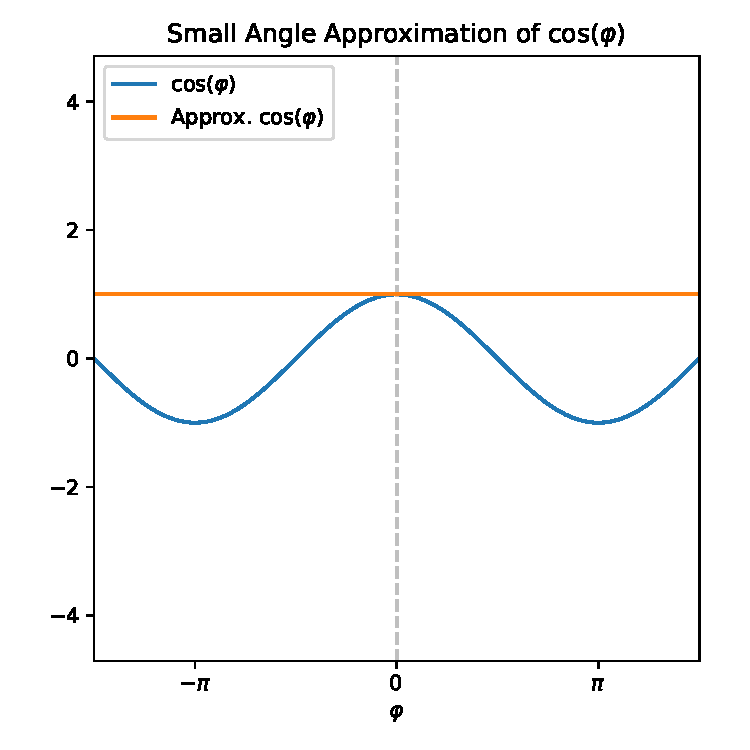
\includegraphics[width = \linewidth]{figures/introduction/generated/small-angle-approximation-cos.pdf}
				\caption{Small angle approximation \( \cos(\varphi) \approx 1 \) of Cosine.}
			\end{subfigure}
			\caption{Visualization of the small angle approximation (given is orange) of the basic trigonometric functions Sine and Cosine (given in blue). It is clear that the approximation is only valid in a small region around zero (\( \varphi \approx 0 \)).}
			\label{fig:smallAngleApproximation}
		\end{figure}

		We now look at two examples of dynamical systems, one which is linear and one that is not.

		\subsection{Harmonic Oscillator}
			\label{subsec:harmonicOscillator}

			\begin{figure}
				\centering
				\tikzHarmonicOscillator
				\caption{Illustration of a simple harmonic oscillator with mass \(m\), spring stiffness \(k\) and position \(x\) that is not affected by any external force like gravity. The mass is in equilibrium if \( x = 0 \).}
				\label{fig:simpleHarmonicOscillator}
			\end{figure}

			The \emph{simple harmonic oscillator} describes the dynamical system of a mass \(m\) that is attached to a spring that is following Hooke's Law with stiffness \(k\) (see~\autoref{fig:simpleHarmonicOscillator}). This harmonic oscillator is described by the \ac{ode}
			\begin{align}
				m\ddot{x} = -kx \quad\iff\quad \ddot{x} = -\frac{k}{m} x  \label{eq:harmonicOscillator}
			\end{align}
			where \(x\) and \(\ddot{x}\) are the position and acceleration of the mass, respectively. Note that if \( x = 0 \), the mass is in equilibrium and no force is acting on it.

			By using basic results in the solution theory of linear \acp{ode}, we see that the general solution is given as
			\begin{align*}
				x(t) = A \cos\Big(t \sqrt{k / m} + \varphi\Big)
			\end{align*}
			with the amplitude \(A\) and the phase \(\varphi\) (see~\autoref{app:harmonicOscillatorSolution} for the derivation of the solution). As neither gravity nor damping or other external forces are involved in the dynamical system, the motion continues forever with a non-changing amplitude.
		% end

		\subsection{Simple Pendulum}
			\label{subsec:simplePendulum}

			\begin{figure}
				\centering
				\tikzSimplePendulum
				\caption{Illustration of an inverse pendulum with mass \(m\) and displacement \(\varphi\) that is only affected by gravity and no other external force. The mass is in equilibrium for both \( \varphi = 0 \) and \( \varphi = \pi \), where the former is an unstable equilibrium.}
				\label{fig:simplePendulum}
			\end{figure}

			The \emph{inverse pendulum} described the dynamical system of a mass \(m\) that is attached to a rigid pole of length \(L\) which can freely swing around a suspension point (see~\autoref{fig:simplePendulum}). The pendulum stands upright if \( \varphi = 0 \) and its equation of motion is described by the \ac{ode}
			\begin{align*}
				\ddot{\varphi} = \frac{g}{L} \sin(\varphi)
			\end{align*}
			where \(g\), \(L\), \(\varphi\) and \(\ddot{\varphi}\) describe the gravity acceleration, pole length, displacement and acceleration of the mass, respectively. Note that if \( \varphi = 0 \), the mass is in an unstable equilibrium and no force is acting on it.

			In comparison to the harmonic oscillator (\autoref{subsec:harmonicOscillator}), this differential equation is nonlinear. And, even for the case with unit gravity acceleration \( g = 1 \) and unit pole length \( L = 1\), where the \ac{ode} looks really simple
			\begin{align}
				\ddot{\varphi} = \sin(\varphi)  \label{eq:inversePendulum}
			\end{align}
			it is not tractable analytically (\ac{ie} there exists no solution in closed form).

			Still, we can apply the small angle approximation introduced before (in this case, \( \sin(\varphi) \approx \varphi \)) which yields the simple equation
			\begin{align}
				\ddot{\varphi} \approx \varphi  \label{eq:linearizedInversePendulum}
			\end{align}
			which is solved by
			\begin{align*}
				\varphi(t) = \frac{1}{2} e^{-t} \big(\varphi_0 + e^{2t} \varphi_0 - \dot{\varphi}_0 + e^{2t} \dot{\varphi}_0\big)
			\end{align*}
			where \(\varphi_0\) and \(\dot{\varphi}_0\) are the initial displacement and velocity, respectively.

			However, this small angle approximation can only forecast small displacements \( \varphi \ll \pi/2 \). And, as the equilibrium at \( \varphi = 0 \) is unstable, the approximation becomes worst and worst as time goes on because the pendulum falls down. This behavior is shown in~\autoref{fig:inversePendulumApprox}.

			\begin{figure}
				\centering
				\begin{subfigure}[t]{0.5\linewidth}
					\centering
					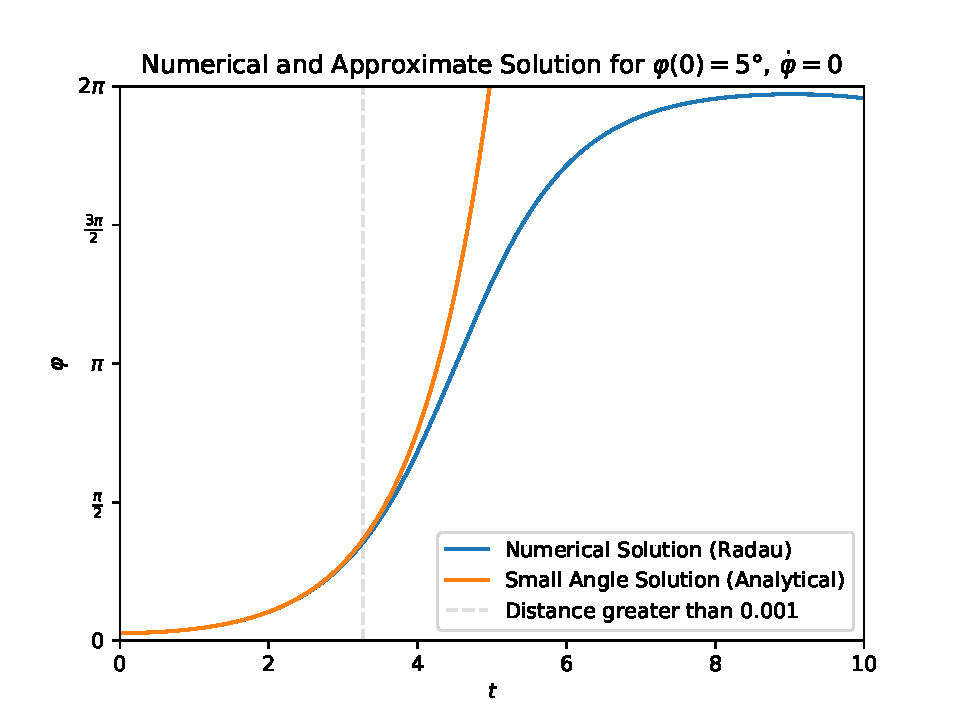
\includegraphics[width = \linewidth]{figures/introduction/generated/pendulum-motion-solutions}
					\caption{Trajectories of two solution strategies to the inverse pendulum, where the blue is a numerical solution of the actual motion of equation (solved using the Radau~IIA method~\cite[72]{hairerSolvingOrdinaryDifferential1996}) and the orange one is the analytically computed solution linearized \ac{ode}. The latter is linearized using small angle approximation. The dotted gray vertical line shows when the distance tolerance of \( \varepsilon = 10^{-3} \) is exceeded.}
				\end{subfigure}%
				~
				\begin{subfigure}[t]{0.5\linewidth}
					\centering
					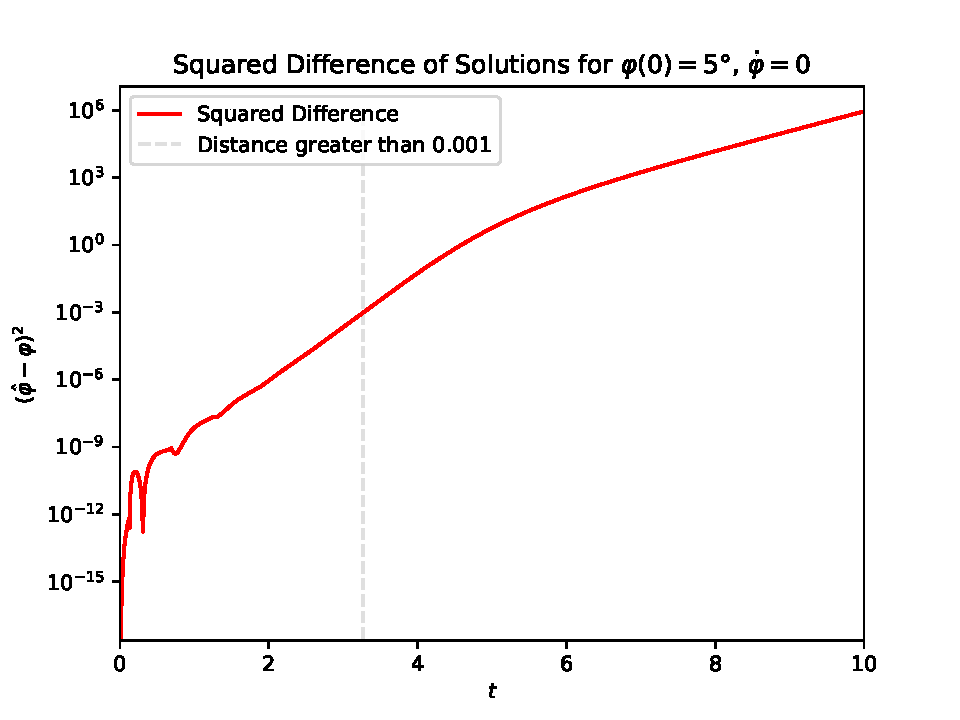
\includegraphics[width = \linewidth]{figures/introduction/generated/pendulum-motion-difference}
					\caption{Differences between the small angle approximation and the numerical solution of the \ac{ode}  The dotted gray vertical line shows when the distance tolerance of \( \varepsilon = 10^{-3} \) is exceeded.}
				\end{subfigure}
				\caption{Comparison of a numerical solution to the \ac{ode} of the inverse pendulum given in\eqref{eq:inversePendulum} and the analytical solution of the linearized \ac{ode} given in\eqref{eq:linearizedInversePendulum}. A tolerance value of \( \varepsilon = 10^{-3} \) is used to show when the both solutions diverge from each other.}
				\label{fig:inversePendulumApprox}
			\end{figure}
		% end
	% end
% end

	\chapter{Experiments}
	\label{c:experiments}

	\todo{Content}
% end

	\chapter{Results}
	\label{c:results}
	\IMRADlabel{results}

	\todo{Results: Content}
% end

	\chapter{Discussion}
	\label{c:discussion}
	\IMRADlabel{discussion}

	\todo{Discussion: Content}
% end

	\chapter{Outlook}
	\label{c:outlook}

	\todo{Outlook: Content}
% end


	\cleardoublepage
	\bibliography{literature/lit}
	\nocite{*}

	\cleardoublepage

	\appendix
	\chapter{Invent some nice chapter title} \todo{Chapter title.}
	\section{Solution of the Harmonic Oscillator}
		\label{app:harmonicOscillatorSolution}
	
		To solve the differential motion equation
		\begin{align*}
			m\ddot{x} = -kx
		\end{align*}
		of the harmonic oscillator given in~\autoref{subsec:harmonicOscillator}, we use the solution approach
		\begin{align*}
			x(t) = c e^{\lambda t} \qquad \dot{x}(t) = \lambda c e^{\lambda t} \qquad \ddot{x}(t) = \lambda^2 c e^{\lambda t}
		\end{align*}
		and insert it into the differential equation:
		\begin{align*}
			m\ddot{x} = -kx \quad\implies\quad
			m \lambda^2 c e^{\lambda t} = -k c e^{\lambda t} \quad\iff\quad
			m \lambda^2 = -k \quad\iff\quad
			\lambda = \pm \sqrt{-\frac{k}{m}}
		\end{align*}
		As both \(k\) and \(m\) are defined to be positive, we get the complex solutions:
		\begin{align*}
			x_1(t) = e^{i t \sqrt{k / m}} \qquad x_2(t) = e^{-i t \sqrt{k / m}}
		\end{align*}
		Due to the superposition principle, also \( x_1 + x_2 \) and \( x_1 - x_2 \) are solutions. Hence, we get two real solutions by using Euler's identity \( e^{\varphi i} = \cos(\varphi) + i \sin(\varphi) \):
		\begin{align*}
			x_1 + x_2
				&= e^{i t \sqrt{k / m}} + e^{-i t \sqrt{k / m}} \\
				&= \cos\Big(t \sqrt{k / m}\Big) + i \sin\Big(t \sqrt{k / m}\Big) + \cos\Big(t \sqrt{k / m}\Big) - i \sin\Big(t \sqrt{k / m}\Big) \\
				&= 2 \cos\Big(t \sqrt{k / m}\Big) \\
			x_1 - x_2
				&= e^{i \sqrt{k / m} t} - e^{-i t \sqrt{k / m}} \\
				&= \cos\Big(t \sqrt{k / m}\Big) i \sin\Big(t \sqrt{k / m}\Big) - \cos\Big(t \sqrt{k / m}\Big) + i \sin\Big(t \sqrt{k / m}\Big) \\
				&=  2i \sin\Big(t \sqrt{k / m}\Big)
		\end{align*}
		This yields the following general solution:
		\begin{align*}
			x(t) = c_1 \cos\Big(t \sqrt{k / m}\Big) + c_2 \sin\Big(t \sqrt{k / m}\Big),\quad c_1, c_2 \in \C
		\end{align*}
		As both Sine and Cosine are Sinusoidal, different \( c_1 \neq c_2 \) only lead to a phase shift. Thus we can also write the solution as
		\begin{align*}
			x(t) = A \cos\Big(t \sqrt{k / m} + \varphi\Big)
		\end{align*}
		with the amplitude \(A\) and the phase \(\varphi\).
	% end
% end

	\chapter{Snippets}
		\section{Linear Dynamical Systems with Nonlinear Measurements}
\label{subsec:slds}



Our idea is to replace the linear measurements \( \vec{y}_t \) in an \ac{lgds}
\begin{align*}
	\vec{s}_{t + 1} & = \mat{A} \vec{s}_t + \vec{w}_t \\
	\vec{y}_t       & = \mat{C} \vec{s}_t + \vec{v}_t
\end{align*}
reported in~\cite{ghahramaniParameterEstimationLinear1996} with an arbitrary, possibly nonlinear but differentiable function \( \vec{g}_{\vec{\theta}} : \R^k \to \R^p \) with characterizing parameters \( \vec{\theta} \). In all of the following, we keep the parameters implicit for brevity.

The vectors \( \vec{w}_t \) and \( \vec{v}_t \) represent the purely additive Gaussian noise of the system (with zero mean and covariance \( \mat{Q} \) and \( \mat{R} \), respectively). Then the states \( \vec{s}_t \), \( \vec{s}_{t - 1} \) and emissions \( \vec{y}_t \) are jointly Gaussian~\cite{minkaHiddenMarkovModels1999}:
\begin{align*}
	p(\vec{s}_t \given \vec{s}_{t - 1}) & \sim \normal(\mat{A} \vec{s}_{t - 1}, \mat{Q})    \\
	p(\vec{y}_t \given \vec{s}_t)       & \sim \normal\big(\vec{g}(\vec{s}_t), \mat{R}\big)
\end{align*}
This model can also be written as a set of both linear and nonlinear equations:
\begin{align*}
	\vec{s}_{t + 1} & = \mat{A} \vec{s}_t + \vec{w}_t  \\
	\vec{w}_t       & \sim \normal(\vec{0}, \mat{Q})   \\
	\vec{y}_t       & = \vec{g}(\vec{s}_t) + \vec{v}_t \\
	\vec{v}_t       & \sim \normal(\vec{0}, \mat{R})
\end{align*}
In all of the following, we assume to have \(N\) \ac{iid} observation sequences. Let \( \vec{y}_{1:T}^{(n)} \) be the \(n\)-th observation sequence and \( \vec{s}_{1:T}^{(n)} \) the corresponding state sequence. All sequences share a single state dynamics matrix, the same noise covariances and observation function. Let \( \vec{y}_{1:T} \coloneqq \big(\vec{y}_{1:T}^{(1)}, \vec{y}_{1:T}^{(2)}, \cdots, \vec{y}_{1:T}^{(N)}\big) \) and \( \vec{s}_{1:T} \coloneqq \big(\vec{s}_{1:T}^{(1)}, \vec{s}_{1:T}^{(2)}, \cdots, \vec{s}_{1:T}^{(n)}\big) \) be the sequences of all observation and state sequences, respectively. The same goes for \( \vec{y}_t \) and \( \vec{s}_t \). We also denote \( \vec{g}_t^{(n)} \coloneqq \vec{g}\big(\vec{s}_t^{(n)}\big) \) for brevity.

\subsection{M-Step}
	For a single observation sequence, the complete log-likelihood \( \ln p\Big(\vec{s}_{1:T}^{(n)}, \vec{y}_{1:T}^{(n)}\Big) \) has the form
	\begin{align*}
		\ln p\Big(\vec{s}_{1:T}^{(n)}, \vec{y}_{1:T}^{(n)}\Big)
			&= \ln \Bigg(\! p\Big(\vec{s}_1^{(n)}\Big) \prod_{t = 2}^{T} p\Big(\vec{s}_t^{(n)} \given \vec{s}_{t - 1}^{(n)}\Big) \prod_{t = 1}^{T} p\Big(\vec{y}_t^{(n)} \given \vec{s}_t^{(n)}\Big) \!\Bigg) \\
			&= \ln p\Big(\vec{s}_1^{(n)}\Big) + \sum_{t = 2}^{T} \ln p\Big(\vec{s}_t^{(n)} \given \vec{s}_{t - 1}^{(n)}\Big) + \sum_{t = 1}^{T} \ln p\Big(\vec{y}_t^{(n)} \given \vec{s}_t^{(n)}\Big) \\
			&= \logGaussianMulti{\vec{s}_1^{(n)}}{\vec{m}_0}{\mat{V}_0}{k} \\
				&\qquad\qquad + \sum_{t = 2}^{T} \logGaussianMulti{\vec{s}_t^{(n)}}{\mat{A} \vec{s}_{t - 1}^{(n)}}{\mat{Q}}{k} \\
				&\qquad\qquad + \sum_{t = 1}^{T} \logGaussianMulti{\vec{y}_t^{(n)}}{\vec{g}_t^{(n)}}{\mat{R}}{p} \\
			&= -\frac{T(k + p)}{2} \ln(2\pi) - \frac{1}{2} \ln \lvert \mat{V}_0 \rvert - \frac{T - 1}{2} \ln \lvert \mat{Q} \rvert - \frac{T}{2} \ln \lvert \mat{R} \rvert \\
				&\qquad\qquad -\frac{1}{2} \Big( \vec{s}_1^{(n)} - \vec{m}_0 \Big)^T \mat{V}_0^{-1} \Big( \vec{s}_1^{(n)} - \vec{m}_0 \Big) \\
				&\qquad\qquad -\frac{1}{2} \sum_{t = 2}^{T} \Big( \vec{s}_t^{(n)} - \mat{A} \vec{s}_{t - 1}^{(n)} \Big)^T \mat{Q}^{-1} \Big( \vec{s}_t^{(n)} - \mat{A} \vec{s}_{t - 1}^{(n)} \Big) \\
				&\qquad\qquad -\frac{1}{2} \sum_{t = 1}^{T} \Big( \vec{y}_t^{(n)} - \vec{g}_t^{(n)} \Big)^T \mat{R}^{-1} \Big( \vec{y}_t^{(n)} - \vec{g}_t^{(n)} \Big)
	\end{align*}
	where \( \vec{m}_0 \) and \( \mat{V}_0 \) are the initial state mean and covariance. As the observation sequences are independent, we can formulate the joint complete log-likelihood \( \ln p(\vec{s}_{1:T}, \vec{y}_{1:T}) \) as the sum of all subsequent log-likelihoods:
	\begin{align*}
		\ln p(\vec{s}_{1:T}, \vec{y}_{1:T})
			&= \ln \prod_{n = 1}^{N} p\Big(\vec{s}_{1:T}^{(n)}, \vec{y}_{1:T}^{(n)}\Big) = \sum_{n = 1}^{N} \ln p\Big(\vec{s}_{1:T}^{(n)}, \vec{y}_{1:T}^{(n)}\Big) \\
			&= -\frac{NT(k + p)}{2} \ln(2\pi) - \frac{N}{2} \ln \lvert \mat{V}_0 \rvert - \frac{N(T - 1)}{2} \ln \lvert \mat{Q} \rvert - \frac{NT}{2} \ln \lvert \mat{R} \rvert \\
				&\qquad\qquad -\frac{1}{2} \sum_{n = 1}^{N} \Big( \vec{s}_1^{(n)} - \vec{m}_0 \Big)^T \mat{V}_0^{-1} \Big( \vec{s}_1^{(n)} - \vec{m}_0 \Big) \\
				&\qquad\qquad -\frac{1}{2} \sum_{n = 1}^{N} \sum_{t = 2}^{T} \Big( \vec{s}_t^{(n)} - \mat{A} \vec{s}_{t - 1}^{(n)} \Big)^T \mat{Q}^{-1} \Big( \vec{s}_t^{(n)} - \mat{A} \vec{s}_{t - 1}^{(n)} \Big) \\
				&\qquad\qquad -\frac{1}{2} \sum_{n = 1}^{N} \sum_{t = 1}^{T} \Big( \vec{y}_t^{(n)} - \vec{g}_t^{(n)} \Big)^T \mat{R}^{-1} \Big( \vec{y}_t^{(n)} - \vec{g}_t^{(n)} \Big)
	\end{align*}

	To derive the M-step formulas, we need to maximize the \emph{expected} complete log-likelihood. Therefore, we will now derive the expected log-likelihood
	\begin{equation*}
		Q = \E\big[ p(\vec{s}_{1:T}, \vec{y}_{1:T}) \given \vec{y}_{1:T} \big]
	\end{equation*}
	This quantity depends on three expectations
	\begin{align*}
		\hat{\vec{s}}_{t \subgiven t_0}^{(n)}  &\coloneqq \E\Big[\vec{s}_t^{(n)} \Biggiven \vec{y}_{1:t_0}\Big]
			& \hat{\vec{s}}_{t \subgiven t_0}           &\coloneqq \frac{1}{N} \sum_{n = 1}^{N} \hat{\vec{s}}_{t \subgiven t_0}^{(n)} \\
		\mat{P}_{t \subgiven t_0}^{(n)}        &\coloneqq \E\bigg[\vec{s}_t^{(n)} \vec{s}_t^{(n), T} \bigggiven \vec{y}_{1:t_0}\bigg]
			& \mat{P}_{t \subgiven t_0}        &\coloneqq \frac{1}{N} \sum_{n = 1}^{N} \mat{P}_{t \subgiven t_0}^{(n)} \\
		\mat{P}_{t, t - 1 \subgiven t_0}^{(n)} &\coloneqq \E\bigg[\vec{s}_t^{(n)} \vec{s}_{t - 1}^{(n), T} \bigggiven \vec{y}_{1:t_0}\bigg]
			& \mat{P}_{t, t - 1 \subgiven t_0} &\coloneqq \frac{1}{N} \sum_{n = 1}^{N} \mat{P}_{t, t - 1 \subgiven t_0}^{(n)}
	\end{align*}
	which form the expected state, self-correlation and cross-correlation, respectively. We call \( \hat{\vec{s}}_{t \subgiven t - 1} \) the prior, \( \hat{\vec{s}}_{t \subgiven t} \) the posterior and \( \hat{\vec{s}}_{t \subgiven T} \) the smoothed states (same for the self- and cross-correlation). For brevity, we also write \( \hat{\vec{s}}_t \) for the smoothed states \( \hat{\vec{s}}_{t \subgiven T} \) (same for the self- and cross-correlation). Additionally we define
	\begin{align}
		\hat{\vec{g}}_t^{(n)} &\coloneqq \E\Big[\vec{g}_t^{(n)} \Biggiven \vec{y}_{1:T}\Big]  \label{eq:expectedMeasurement} \\
		\mat{G}_t^{(n)}       &\coloneqq \E\Big[\vec{g}_t^{(n)} \vec{g}_t^{(n), T} \Biggiven \vec{y}_{1:T}\Big]  \label{eq:expectedMeasurementMat}
	\end{align}
	to be the expectations of the measurement function \( \vec{g}_t^{(n)} \). We will see that evaluating this expectation is not possible in a closed form and has to be approximated, but for now we will be deriving the expected complete log-likelihood dependent on the defined expectations.

	For simplicity, let
	\begin{align*}
		q_1 &\coloneqq -\frac{NT(k + p)}{2} \ln(2\pi) - \frac{N}{2} \ln \lvert \mat{V}_0 \rvert - \frac{N(T - 1)}{2} \ln \lvert \mat{Q} \rvert - \frac{NT}{2} \ln \lvert \mat{R} \rvert \\
		q_2 &\coloneqq -\frac{1}{2} \sum_{n = 1}^{N} \Big( \vec{s}_1^{(n)} - \vec{m}_0 \Big)^T \mat{V}_0^{-1} \Big( \vec{s}_1^{(n)} - \vec{m}_0 \Big) \\
		q_3 &\coloneqq -\frac{1}{2} \sum_{n = 1}^{N} \sum_{t = 2}^{T} \Big( \vec{s}_t^{(n)} - \mat{A} \vec{s}_{t - 1}^{(n)} \Big)^T \mat{Q}^{-1} \Big( \vec{s}_t^{(n)} - \mat{A} \vec{s}_{t - 1}^{(n)} \Big) \\
		q_4 &\coloneqq -\frac{1}{2} \sum_{n = 1}^{N} \sum_{t = 1}^{T} \Big( \vec{y}_t^{(n)} - \vec{g}_t^{(n)} \Big)^T \mat{R}^{-1} \Big( \vec{y}_t^{(n)} - \vec{g}_t^{(n)} \Big)
	\end{align*}
	such that \( \ln p(\vec{s}_{1:T}, \vec{y}_{1:T}) = q_1 + q_2 + q_3 + q_4 \) and, with \(Q_1\), \(Q_2\), \(Q_3\) and \(Q_4\) being the corresponding expectations, \( Q = Q_1 + Q_2 + Q_3 + Q_4 \).

	We start with \(Q_1\):
	\begin{equation*}
		Q_1 = \E[q_1 \given \vec{y}_{1:T}] = -\frac{NT(k + p)}{2} \ln(2\pi) - \frac{N}{2} \ln \lvert \mat{V}_0 \rvert - \frac{N(T - 1)}{2} \ln \lvert \mat{Q} \rvert - \frac{NT}{2} \ln \lvert \mat{R} \rvert
	\end{equation*}
	Then following \(Q_2\):
	\begin{align*}
		Q_2
			&= \E[q_2 \given \vec{y}_{1:T}] \\
			&= \E\Bigg[\! -\frac{1}{2} \sum_{n = 1}^{N} \Big( \vec{s}_1^{(n)} - \vec{m}_0 \Big)^T \mat{V}_0^{-1} \Big( \vec{s}_1^{(n)} - \vec{m}_0 \Big) \Bigggiven \vec{y}_{1:T} \Bigg] \\
			&= -\frac{1}{2} \sum_{n = 1}^{N} \E\Bigg[ \Big( \vec{s}_1^{(n)} - \vec{m}_0 \Big)^T \mat{V}_0^{-1} \Big( \vec{s}_1^{(n)} - \vec{m}_0 \Big) \Bigggiven \vec{y}_{1:T} \Bigg] \\
			&= -\frac{1}{2} \sum_{n = 1}^{N} \E\Bigg[ \tr\!\bigg(\!\Big( \vec{s}_1^{(n)} - \vec{m}_0 \Big)^T \mat{V}_0^{-1} \Big( \vec{s}_1^{(n)} - \vec{m}_0 \Big)\!\bigg) \Bigggiven \vec{y}_{1:T} \Bigg] \\
			&= -\frac{1}{2} \sum_{n = 1}^{N} \E\Bigg[ \tr\!\bigg(\!\Big( \vec{s}_1^{(n)} - \vec{m}_0 \Big) \Big( \vec{s}_1^{(n)} - \vec{m}_0 \Big)^T \mat{V}_0^{-1} \!\bigg) \Bigggiven \vec{y}_{1:T} \Bigg] \\
			&= -\frac{1}{2} \sum_{n = 1}^{N} \E\Bigg[ \tr\!\bigg(\!\Big( \vec{s}_1^{(n)} - \vec{m}_0 \Big) \Big( \vec{s}_1^{(n), T} - \vec{m}_0^T \Big) \mat{V}_0^{-1} \!\bigg) \Bigggiven \vec{y}_{1:T} \Bigg] \\
			&= -\frac{1}{2} \sum_{n = 1}^{N} \E\Bigg[ \tr\!\bigg(\! \Big( \vec{s}_1^{(n)} \vec{s}_1^{(n), T} - \vec{s}_1^{(n)} \vec{m}_0^T - \vec{m} \vec{s}_1^{(n), T} + \vec{m}_0 \vec{m}_0^T \Big) \mat{V}_0^{-1} \!\bigg) \Bigggiven \vec{y}_{1:T} \Bigg] \\
			&= -\frac{1}{2} \sum_{n = 1}^{N} \tr\!\Big( \mat{P}_1^{(n)} \mat{V}_0^{-1} - \hat{\vec{s}}_1^{(n)} \vec{m}_0^T \mat{V}_0^{-1} - \vec{m} \hat{\vec{s}}_1^{(n), T} \mat{V}_0^{-1} + \vec{m}_0 \vec{m}_0^T \mat{V}_0^{-1} \Big) \\
			&= -\frac{1}{2} \sum_{n = 1}^{N} \tr\!\Big( \mat{P}_1^{(n)} \mat{V}_0^{-1} \Big) - \tr\!\Big( \hat{\vec{s}}_1^{(n)} \vec{m}_0^T \mat{V}_0^{-1} \Big) - \tr\!\Big( \vec{m}_0 \hat{\vec{s}}_1^{(n), T} \mat{V}_0^{-1} \Big) + \tr\!\Big(\vec{m}_0 \vec{m}_0^T \mat{V}_0^{-1} \Big) \\
			&=  -\frac{N}{2} \tr\!\Big( \mat{P}_1 \mat{V}_0^{-1} \Big) + \frac{N}{2} \tr\!\Big( \hat{\vec{s}}_1 \vec{m}_0^T \mat{V}_0^{-1} \Big) + \frac{N}{2} \tr\!\Big( \vec{m}_0 \hat{\vec{s}}_1^T \mat{V}_0^{-1} \Big) - \frac{N}{2} \tr\!\Big(\vec{m}_0 \vec{m}_0^T \mat{V}_0^{-1} \Big)
	\end{align*}
	And \(Q_3\):
	\begin{align*}
		Q_3
			&= \E[q_3 \given \vec{y}_{1:T}] \\
			&= \E\Bigg[\! -\frac{1}{2} \sum_{n = 1}^{N} \sum_{t = 2}^{T} \Big( \vec{s}_t^{(n)} - \mat{A} \vec{s}_{t - 1}^{(n)} \Big)^T \mat{Q}^{-1} \Big( \vec{s}_t^{(n)} - \mat{A} \vec{s}_{t - 1}^{(n)} \Big) \Bigggiven \vec{y}_{1:T} \Bigg] \\
			&= -\frac{1}{2} \sum_{n = 1}^{N} \sum_{t = 2}^{T} \E\Bigg[ \Big( \vec{s}_t^{(n)} - \mat{A} \vec{s}_{t - 1}^{(n)} \Big)^T \mat{Q}^{-1} \Big( \vec{s}_t^{(n)} - \mat{A} \vec{s}_{t - 1}^{(n)} \Big) \Bigggiven \vec{y}_{1:T} \Bigg] \\
			&= -\frac{1}{2} \sum_{n = 1}^{N} \sum_{t = 2}^{T} \E\Bigg[ \tr\!\bigg(\!\Big( \vec{s}_t^{(n)} - \mat{A} \vec{s}_{t - 1}^{(n)} \Big)^T \mat{Q}^{-1} \Big( \vec{s}_t^{(n)} - \mat{A} \vec{s}_{t - 1}^{(n)} \Big)\!\bigg) \Bigggiven \vec{y}_{1:T} \Bigg] \\
			&= -\frac{1}{2} \sum_{n = 1}^{N} \sum_{t = 2}^{T} \E\Bigg[ \tr\!\bigg(\!\Big( \vec{s}_t^{(n)} - \mat{A} \vec{s}_{t - 1}^{(n)} \Big) \Big( \vec{s}_t^{(n)} - \mat{A} \vec{s}_{t - 1}^{(n)} \Big)^T \mat{Q}^{-1} \!\bigg) \Bigggiven \vec{y}_{1:T} \Bigg] \\
			&= -\frac{1}{2} \sum_{n = 1}^{N} \sum_{t = 2}^{T} \E\Bigg[ \tr\!\bigg(\!\Big( \vec{s}_t^{(n)} - \mat{A} \vec{s}_{t - 1}^{(n)} \Big) \Big(\vec{s}_t^{(n), T} - \vec{s}_{t - 1}^{(n), T} \mat{A}^T \Big) \mat{Q}^{-1} \!\bigg) \Bigggiven \vec{y}_{1:T} \Bigg] \\
			&= -\frac{1}{2} \sum_{n = 1}^{N} \sum_{t = 2}^{T} \E\Bigg[ \tr\!\bigg(\!\Big( \vec{s}_t^{(n)} \vec{s}_t^{(n), T} - \vec{s}_t^{(n)} \vec{s}_{t - 1}^{(n), T} \mat{A}^T - \mat{A} \vec{s}_{t - 1}^{(n)} \vec{s}_t^{(n), T} - \mat{A} \vec{s}_{t - 1}^{(n)} \vec{s}_{t - 1}^{(n), T} \mat{A}^T \Big) \mat{Q}^{-1} \!\bigg) \Bigggiven \vec{y}_{1:T} \Bigg] \\
			&= -\frac{1}{2} \sum_{n = 1}^{N} \sum_{t = 2}^{T} \tr\!\Big( \mat{P}_t^{(n)} \mat{Q}^{-1} - \mat{P}_{t, t - 1}^{(n)} \mat{A}^T \mat{Q}^{-1} - \mat{A} \underbrace{\mat{P}_{t - 1, t}^{(n)}}_{=\, \mat{P}_{t, t - 1}^{(n)}} \mat{Q}^{-1} - \mat{A} \mat{P}_{t - 1}^{(n)} \mat{A}^T \mat{Q}^{-1} \Big) \\
			&= -\frac{1}{2} \sum_{n = 1}^{N} \sum_{t = 2}^{T} \tr\!\Big( \mat{P}_t^{(n)} \mat{Q}^{-1} \Big) - \tr\!\Big( \mat{P}_{t, t - 1}^{(n)} \mat{A}^T \mat{Q}^{-1} \Big) - \tr\!\Big( \mat{A} \mat{P}_{t, t - 1}^{(n)} \mat{Q}^{-1} \Big) - \tr\!\Big( \mat{A} \mat{P}_{t - 1}^{(n)} \mat{A}^T \mat{Q}^{-1} \Big) \\
			&= -\frac{N}{2} \sum_{t = 2}^{T} \tr\!\Big( \mat{P}_t \mat{Q}^{-1} \Big) - \tr\!\Big( \mat{P}_{t, t - 1} \mat{A}^T \mat{Q}^{-1} \Big) - \tr\!\Big( \mat{A} \mat{P}_{t, t - 1} \mat{Q}^{-1} \Big) - \tr\!\Big( \mat{A} \mat{P}_{t - 1} \mat{A}^T \mat{Q}^{-1} \Big)
	\end{align*}
	Finally, we derive \(Q_4\). This is the one that depends on the non-closed-form expectations~\eqref{eq:expectedMeasurement} and~\eqref{eq:expectedMeasurementMat}:
	\begin{align*}
		Q_4
			&= \E[q_4 \given \vec{y}_{1:T}] \\
			&= \E\Bigg[\! -\frac{1}{2} \sum_{n = 1}^{N} \sum_{t = 1}^{T} \Big( \vec{y}_t^{(n)} - \vec{g}_t^{(n)} \Big)^T \mat{R}^{-1} \Big( \vec{y}_t^{(n)} - \vec{g}_t^{(n)} \Big) \bigggiven \vec{y}_{1:T} \Bigg] \\
			&= -\frac{1}{2} \sum_{n = 1}^{N} \sum_{t = 1}^{T} \E\Bigg[ \Big( \vec{y}_t^{(n)} - \vec{g}_t^{(n)} \Big)^T \mat{R}^{-1} \Big( \vec{y}_t^{(n)} - \vec{g}_t^{(n)} \Big) \bigggiven \vec{y}_{1:T} \Bigg] \\
			&= -\frac{1}{2} \sum_{n = 1}^{N} \sum_{t = 1}^{T} \E\Bigg[ \tr\!\bigg(\!\Big( \vec{y}_t^{(n)} - \vec{g}_t^{(n)} \Big)^T \mat{R}^{-1} \Big( \vec{y}_t^{(n)} - \vec{g}_t^{(n)} \Big)\!\bigg) \bigggiven \vec{y}_{1:T} \Bigg] \\
			&= -\frac{1}{2} \sum_{n = 1}^{N} \sum_{t = 1}^{T} \E\Bigg[ \tr\!\bigg(\!\Big( \vec{y}_t^{(n)} - \vec{g}_t^{(n)} \Big) \Big( \vec{y}_t^{(n)} - \vec{g}_t^{(n)} \Big)^T \mat{R}^{-1} \!\bigg) \bigggiven \vec{y}_{1:T} \Bigg] \\
			&= -\frac{1}{2} \sum_{n = 1}^{N} \sum_{t = 1}^{T} \E\Bigg[ \tr\!\bigg(\!\Big( \vec{y}_t^{(n)} - \vec{g}_t^{(n)} \Big) \Big( \vec{y}_t^{(n), T} - \vec{g}_t^{(n), T} \Big) \mat{R}^{-1} \!\bigg) \bigggiven \vec{y}_{1:T} \Bigg] \\
			&= -\frac{1}{2} \sum_{n = 1}^{N} \sum_{t = 1}^{T} \E\Bigg[ \tr\!\bigg(\!\Big( \vec{y}_t^{(n)} \vec{y}_t^{(n), T} - \vec{y}_t^{(n)} \vec{g}_t^{(n), T} - \vec{g}_t^{(n)} \vec{y}_t^{(n), T} + \vec{g}_t^{(n)} \vec{g}_t^{(n), T} \Big) \mat{R}^{-1} \!\bigg) \bigggiven \vec{y}_{1:T} \Bigg] \\
			&= -\frac{1}{2} \sum_{n = 1}^{N} \sum_{t = 1}^{T} \tr\!\Big( \vec{y}_t^{(n)} \vec{y}_t^{(n), T} \mat{R}^{-1} - \vec{y}_t^{(n)} \hat{\vec{g}}_t^{(n), T} \mat{R}^{-1} - \hat{\vec{g}}_t^{(n)} \vec{y}_t^{(n), T} \mat{R}^{-1} + \mat{G}_t^{(n)} \mat{R}^{-1} \Big) \\
			&= -\frac{1}{2} \sum_{n = 1}^{N} \sum_{t = 1}^{T} \tr\!\Big( \vec{y}_t^{(n)} \vec{y}_t^{(n), T} \mat{R}^{-1} \Big) - \tr\!\Big( \vec{y}_t^{(n)} \hat{\vec{g}}_t^{(n), T} \mat{R}^{-1} \Big) - \tr\!\Big( \hat{\vec{g}}_t^{(n)} \vec{y}_t^{(n), T} \mat{R}^{-1} \Big) + \tr\!\Big( \mat{G}_t^{(n)} \mat{R}^{-1} \Big)
	\end{align*}

	Putting it all together, the expected complete log-likelihood across all observation sequences is given as
	\begin{align*}
		Q
			&= Q_1 + Q_2 + Q_3 + Q_4 \\
			&= -\frac{NT(k + p)}{2} \ln(2\pi) - \frac{N}{2} \ln \lvert \mat{V}_0 \rvert - \frac{N(T - 1)}{2} \ln \lvert \mat{Q} \rvert - \frac{NT}{2} \ln \lvert \mat{R} \rvert \\
				&\qquad\qquad -\frac{N}{2} \tr\!\Big( \mat{P}_1 \mat{V}_0^{-1} \Big) + \frac{N}{2} \tr\!\Big( \hat{\vec{s}}_1 \vec{m}_0^T \mat{V}_0^{-1} \Big) + \frac{N}{2} \tr\!\Big( \vec{m}_0 \hat{\vec{s}}_1^T \mat{V}_0^{-1} \Big) - \frac{N}{2} \tr\!\Big(\vec{m}_0 \vec{m}_0^T \mat{V}_0^{-1} \Big) \\
				&\qquad\qquad -\frac{N}{2} \sum_{t = 2}^{T} \tr\!\Big( \mat{P}_t \mat{Q}^{-1} \Big) - \tr\!\Big( \mat{P}_{t, t - 1} \mat{A}^T \mat{Q}^{-1} \Big) - \tr\!\Big( \mat{A} \mat{P}_{t, t - 1} \mat{Q}^{-1} \Big) - \tr\!\Big( \mat{A} \mat{P}_{t - 1} \mat{A}^T \mat{Q}^{-1} \Big) \\
				&\qquad\qquad -\frac{1}{2} \sum_{n = 1}^{N} \sum_{t = 1}^{T} \tr\!\Big( \vec{y}_t^{(n)} \vec{y}_t^{(n), T} \mat{R}^{-1} \Big) - \tr\!\Big( \vec{y}_t^{(n)} \hat{\vec{g}}_t^{(n), T} \mat{R}^{-1} \Big) - \tr\!\Big( \hat{\vec{g}}_t^{(n)} \vec{y}_t^{(n), T} \mat{R}^{-1} \Big) + \tr\!\Big( \mat{G}_t^{(n)} \mat{R}^{-1} \Big)
	\end{align*}
	where \( Q_1 \), \( Q_2 \), \( Q_3 \) and \( Q_4 \) are functions of the parameters \( \mat{A} \), \( \mat{Q} \), \( \vec{\theta} \), \( \mat{R} \), \( \vec{m}_0 \) and \( \mat{V}_0 \):
	\begin{align*}
		Q_1 & = Q_1(\mat{V}_0, \mat{Q}, \mat{R}) \\
		Q_2 & = Q_2(\vec{m}_0, \mat{V}_0)        \\
		Q_3 & = Q_3(\mat{A}, \mat{Q})            \\
		Q_4 & = Q_4(\vec{\theta}, \mat{R})
	\end{align*}

	Now we have everything together to derive the M-step equations by maximizing \(Q\). To maximize \(Q\) \ac{wrt} all parameters, that is
	\begin{itemize}
		\item state dynamics matrix \(\mat{A}\),
		\item state noise covariance \(\mat{Q}\),
		\item measurement function parameters \(\vec{\theta}\),
		\item measurement noise covariance \(\mat{R}\),
		\item initial state mean \(\vec{m}_0\) and
		\item initial state covariance \(\mat{V}_0\),
	\end{itemize}
	we have to take the derivatives \ac{wrt} to all the above parameters and set them to zero.
	\begin{itemize}
		\item State dynamics matrix \(\mat{A}\):
	\end{itemize}
	\begin{align}
		&&\pdv{Q}{\mat{A}}
			&= \pdv{Q_1}{\mat{A}} + \pdv{Q_2}{\mat{A}} + \pdv{Q_3}{\mat{A}} + \pdv{Q_4}{\mat{A}} = \pdv{Q_3}{\mat{A}} & \nonumber \\
		&&	&= -\frac{N}{2} \sum_{t = 2}^{T} -\mat{Q}^{-1} \mat{P}_{t, t - 1} - \mat{Q}^{-T} \mat{P}_{t, t - 1}^T + \mat{Q}^{-T} \mat{A} \mat{P}_{t - 1}^T + \mat{Q}^{-1} \mat{A} \mat{P}_{t - 1} & \nonumber \\
		&&	&\oversetfootnotemark{=} -N \sum_{t = 2}^{T} -\mat{Q}^{-1} \mat{P}_{t, t - 1} + \mat{Q}^{-1} \mat{A} \mat{P}_{t - 1} \overset{!}{=} \mat{0} & \nonumber \\
		\implies && \mat{A}^\new &= \Bigg(\! \sum_{t = 2}^{T} \mat{P}_{t, t - 1} \!\Bigg) \Bigg(\! \sum_{t = 2}^{T} \mat{P}_{t - 1} \!\Bigg)^{-1} & \label{eq:stateDynamicsMatrix}
	\end{align}
	\footnotetext{Covariance and correlation matrices (\( \mat{Q} \), \( \mat{R} \), \( \mat{P}_t \), \( \mat{P}_{t, t - 1} \)) are symmetric by definition.}

	\begin{itemize}
		\item State noise covariance \(\mat{Q}\): \\ Instead of maximizing \ac{wrt} \(\mat{Q}\), we can also minimize \ac{wrt} \(\mat{Q}^{-1}\) which has the same effect.
	\end{itemize}
	\begin{align}
		&&\pdv{Q}{\mat{Q}^{-1}}
			&= \pdv{Q_1}{\mat{Q}^{-1}} + \pdv{Q_2}{\mat{Q}^{-1}} + \pdv{Q_3}{\mat{Q}^{-1}} + \pdv{Q_4}{\mat{Q}^{-1}} = \pdv{Q_1}{\mat{Q}^{-1}} + \pdv{Q_3}{\mat{Q}^{-1}} & \nonumber \\
		&&	&\oversetfootnotemark{=} \frac{N(T - 1)}{2} \mat{Q} - \frac{N}{2} \sum_{t = 2}^{T} \mat{P}_t^T - \mat{A} \mat{P}_{t, t - 1}^T - \mat{P}_{t, t - 1}^T \mat{A}^T + \mat{A} \mat{P}_{t - 1}^T \mat{A}^T & \nonumber \\
		&&	&= \frac{N(T - 1)}{2} \mat{Q} - \frac{N}{2} \sum_{t = 2}^{T} \mat{P}_t - \mat{A} \mat{P}_{t, t - 1} - \mat{P}_{t, t - 1} \mat{A}^T + \mat{A} \mat{P}_{t - 1} \mat{A}^T & \nonumber \\
		&&	&= \frac{N(T - 1)}{2} \mat{Q} - \frac{N}{2} \sum_{t = 2}^{T} \mat{P}_t + \frac{N}{2} \sum_{t = 2}^{T} \mat{A} \mat{P}_{t, t - 1} + \frac{N}{2} \sum_{t = 2}^{T} \mat{P}_{t, t - 1} \mat{A}^T - \frac{N}{2} \sum_{t = 2}^{T} \mat{A} \mat{P}_{t - 1} \mat{A}^T & \nonumber \\
		&&	&= \frac{N(T - 1)}{2} \mat{Q} - \frac{N}{2} \sum_{t = 2}^{T} \mat{P}_t + \frac{N}{2} \mat{A}^\new \sum_{t = 2}^{T} \mat{P}_{t, t - 1} + \frac{N}{2} \Bigg(\! \sum_{t = 2}^{T} \mat{P}_{t, t - 1} \!\Bigg) \big(\mat{A}^\new\big)^T & \nonumber \\
			&&	&\qquad\qquad - \frac{N}{2} \mat{A}^\new \Bigg(\! \sum_{t = 2}^{T} \mat{P}_{t - 1} \!\Bigg) \big(\mat{A}^\new\big)^T & \nonumber \\
		&&	&= \frac{N(T - 1)}{2} \mat{Q} - \frac{N}{2} \sum_{t = 2}^{T} \mat{P}_t + \frac{N}{2} \mat{A}^\new \sum_{t = 2}^{T} \mat{P}_{t, t - 1} + \frac{N}{2} \Bigg(\! \sum_{t = 2}^{T} \mat{P}_{t, t - 1} \!\Bigg) \Bigg(\! \sum_{t = 2}^{T} \mat{P}_{t - 1} \!\Bigg)^{-T} \Bigg(\! \sum_{t = 2}^{T} \mat{P}_{t, t - 1} \!\Bigg)^T & \nonumber \\
			&&	&\qquad\qquad - \frac{N}{2} \Bigg(\! \sum_{t = 2}^{T} \mat{P}_{t, t - 1} \!\Bigg) \Bigg(\! \sum_{t = 2}^{T} \mat{P}_{t - 1} \!\Bigg)^{-1} \Bigg(\! \sum_{t = 2}^{T} \mat{P}_{t - 1} \!\Bigg) \Bigg(\! \sum_{t = 2}^{T} \mat{P}_{t - 1} \!\Bigg)^{-T} \Bigg(\! \sum_{t = 2}^{T} \mat{P}_{t, t - 1} \!\Bigg)^T & \nonumber \\
		&&	&= \frac{N(T - 1)}{2} \mat{Q} - \frac{N}{2} \sum_{t = 2}^{T} \mat{P}_t + \frac{N}{2} \mat{A}^\new \sum_{t = 2}^{T} \mat{P}_{t, t - 1} + \frac{N}{2} \Bigg(\! \sum_{t = 2}^{T} \mat{P}_{t, t - 1} \!\Bigg) \Bigg(\! \sum_{t = 2}^{T} \mat{P}_{t - 1} \!\Bigg)^{-1} \Bigg(\! \sum_{t = 2}^{T} \mat{P}_{t, t - 1} \!\Bigg) & \nonumber \\
			&&	&\qquad\qquad - \frac{N}{2} \Bigg(\! \sum_{t = 2}^{T} \mat{P}_{t, t - 1} \!\Bigg) \Bigg(\! \sum_{t = 2}^{T} \mat{P}_{t - 1} \!\Bigg)^{-1} \cancel{\Bigg(\! \sum_{t = 2}^{T} \mat{P}_{t - 1} \!\Bigg) \Bigg(\! \sum_{t = 2}^{T} \mat{P}_{t - 1} \!\Bigg)^{-1}} \Bigg(\! \sum_{t = 2}^{T} \mat{P}_{t, t - 1} \!\Bigg) & \nonumber \\
		&&	&= \frac{N(T - 1)}{2} \mat{Q} - \frac{N}{2} \Bigg(\! \sum_{t = 2}^{T} \mat{P}_t - \mat{A}^\new \sum_{t = 2}^{T} \mat{P}_{t, t - 1} \!\Bigg) \overset{!}{=} \mat{0} & \nonumber \\
		\implies && \mat{Q}^\new &= \frac{1}{T - 1} \Bigg(\! \sum_{t = 2}^{T} \mat{P}_t - \mat{A}^\new \sum_{t = 2}^{T} \mat{P}_{t, t - 1} \!\Bigg) & \label{eq:stateNoiseCovariance}
	\end{align}
	\footnotetext{Note that \( \pdv{\mat{Q}^{-1}} \ln \det \mat{Q} = \pdv{\mat{Q}^{-1}} \ln \det \big(\mat{Q}^{-1}\big)^{-1} = \bigg( \pdv{\det (\mat{Q}^{-1})^{-1}} \ln \det \big(\mat{Q}^{-1}\big)^{-1} \bigg) \bigg( \pdv{\mat{Q}^{-1}} \det \big(\mat{Q}^{-1}\big)^{-1} \bigg) \overset{\text{cov. matrix}}{=} -\mat{Q} \)}

	\begin{itemize}
		\item Initial state mean \(\vec{m}_0\):
	\end{itemize}
	\begin{align}
		&&\pdv{Q}{\vec{m}_0}
			&= \pdv{Q_1}{\vec{m}_0} + \pdv{Q_2}{\vec{m}_0} + \pdv{Q_3}{\vec{m}_0} + \pdv{Q_4}{\vec{m}_0} = \pdv{Q_2}{\vec{m}_0} & \nonumber \\
		&&	&= \frac{N}{2} \mat{V}_0^{-1} \hat{\vec{s}}_1 + \frac{N}{2} \mat{V}_0^{-T} \hat{\vec{s}}_1 - \frac{N}{2} \big( \mat{V}_0^{-1} \vec{m}_0 + \mat{V}_0^{-T} \vec{m}_0 \big) & \nonumber \\
		&&	&= N \mat{V}_0^{-1} \hat{\vec{s}}_1 - N \mat{V}_0^{-1} \vec{m}_0 & \nonumber \\
		&&	&= N \mat{V}_0^{-1} \big( \hat{\vec{s}}_1 - \vec{m}_0 \big) \overset{!}{=} \vec{0} & \nonumber \\
		\implies && \vec{m}_0^\new &= \hat{\vec{s}}_1 = \frac{1}{N} \sum_{n = 1}^{N} \hat{\vec{s}}_1^{(n)} & \label{eq:initialStateMean}
	\end{align}

	\begin{itemize}
		\item Initial state covariance \(\mat{V}_0\):
	\end{itemize}
	\begin{align}
		&&\pdv{Q}{\mat{V}_0^{-1}}
			&= \pdv{Q_1}{\mat{V}_0^{-1}} + \pdv{Q_2}{\mat{V}_0^{-1}} + \pdv{Q_3}{\mat{V}_0^{-1}} + \pdv{Q_4}{\mat{V}_0^{-1}} = \pdv{Q_1}{\mat{V}_0^{-1}} + \pdv{Q_2}{\mat{V}_0^{-1}} & \nonumber \\
		&&	&= \frac{N}{2} \mat{V}_0 - \frac{N}{2} \mat{P}_1^T + \frac{N}{2} \vec{m}_0 \hat{\vec{s}}_1^T + \frac{N}{2} \hat{\vec{s}}_1 \vec{m}_0^T - \frac{N}{2} \vec{m}_0 \vec{m}_0^T & \nonumber \\
		&&	&= \frac{N}{2} \mat{V}_0 - \frac{N}{2} \mat{P}_1^T + \frac{N}{2} \hat{\vec{s}}_1 \hat{\vec{s}}_1^T + \frac{N}{2} \hat{\vec{s}}_1 \hat{\vec{s}}_1^T - \frac{N}{2} \hat{\vec{s}}_1 \hat{\vec{s}}_1^T & \nonumber \\
		&&	&= \frac{N}{2} \mat{V}_0 - \frac{N}{2} \mat{P}_1^T + \frac{N}{2} \hat{\vec{s}}_1 \hat{\vec{s}}_1^T \overset{!}{=} \mat{0} & \nonumber \\
		\implies && \mat{V}_0^\new &= \mat{P}_1 - \hat{\vec{s}}_1 \hat{\vec{s}}_1^T & \label{eq:initialStateCovariance}
	\end{align}

	\begin{itemize}
		\item Measurement noise covariance \(\mat{R}\):
	\end{itemize}
	\begin{align}
		&&\pdv{Q}{\mat{R}^{-1}}
			&= \pdv{Q_1}{\mat{R}^{-1}} + \pdv{Q_2}{\mat{R}^{-1}} + \pdv{Q_3}{\mat{R}^{-1}} + \pdv{Q_4}{\mat{R}^{-1}} = \pdv{Q_1}{\mat{R}^{-1}} + \pdv{Q_4}{\mat{R}^{-1}} & \nonumber \\
		&&	&= \frac{NT}{2} \mat{R} - \frac{1}{2} \sum_{n = 1}^{N} \sum_{t = 1}^{T} \vec{y}_t^{(n)} \vec{y}_t^{(n), T} - \hat{\vec{g}}_t^{(n)} \vec{y}_t^{(n), T} - \vec{y}_t^{(n)} \hat{\vec{g}}_t^{(n), T} + \mat{G}_t^{(n), T} \overset{!}{=} \mat{0} & \nonumber \\
		\implies && \mat{R}^\new &= \frac{1}{NT} \sum_{n = 1}^{N} \sum_{t = 1}^{T} \vec{y}_t^{(n)} \vec{y}_t^{(n), T} - \hat{\vec{g}}_t^{(n)} \vec{y}_t^{(n), T} - \vec{y}_t^{(n)} \hat{\vec{g}}_t^{(n), T} + \mat{G}_t^{(n), T} & \label{eq:measurementNoiseCovariance}
	\end{align}

	The equations for the state dynamics matrix~\eqref{eq:stateDynamicsMatrix}, the state noise covariance~\eqref{eq:stateNoiseCovariance}, the initial state mean~\eqref{eq:initialStateMean} and the initial state covariance~\eqref{eq:initialStateCovariance} match exactly the equations given in~\cite{ghahramaniParameterEstimationLinear1996}. The equation for the measurement noise covariance~\eqref{eq:measurementNoiseCovariance} differs from the one given in~\cite{ghahramaniParameterEstimationLinear1996} as we are having nonlinear measurements and thus we cannot write the covariance in such a compact form.

	As said before, the expectations~\eqref{eq:expectedMeasurement} and~\eqref{eq:expectedMeasurementMat} are problematic as we cannot evaluate the integrals
	\begin{align*}
		\hat{\vec{g}}_t^{(n)} &= \int\! \vec{g}_t^{(n)} p\Big(\vec{s}_t^{(n)} \Biggiven \vec{y}_{1:T}\Big) \dd{\vec{s}_{1:T}^{(n)}} \\
		\mat{G}_t^{(n)}       &= \int\! \vec{g}_t^{(n)} \vec{g}\vec{s}_t^{(n), T} p\Big(\vec{s}_t^{(n)} \Biggiven \vec{y}_{1:T} \Big) \dd{\vec{s}_{1:T}^{(n)}}
	\end{align*}
	in closed form (the function \( \vec{g}(\cdot) \) is nonlinear). Note that the posterior distribution is Gaussian
	\begin{equation*}
		p\Big(\vec{s}_t^{(n)} \Biggiven \vec{y}_{1:T}\Big) \sim \normal\Big(\hat{\vec{s}}_{t}^{(n)}, \mat{V}_t^{(n)}\Big)
	\end{equation*}
	where \( \hat{\vec{s}}_{t}^{(n)} \) and \( \mat{V}_{t} \) form the posterior mean and covariance, respectively. These are calculated in the E-step (formulas~\eqref{eq:posteriorMean} and~\eqref{eq:posteriorCov}). Due to this Gaussian behavior, we can approximate the integrals using the spherical-radial cubature rule~\cite{solinCubatureIntegrationMethods2010} given in equation~\eqref{eq:sphericalRadialGaussianCubatureRule} (with \( \vec{\xi}_i = \sqrt{k} [\vec{1}]_i \)):
	\begin{align}
		\int\! \vec{g}_t^{(n)} p\Big(\vec{s}_t^{(n)} \Biggiven \vec{y}_{1:T}\Big) \dd{\vec{s}_t^{(n)}}
			&\approx \frac{1}{2k} \sum_{i = 1}^{2k} \vec{g}\Big(\!\sqrt{\mat{V}_t^{(n)}} \vec{\xi}_i + \hat{\vec{s}}_t^{(n)}\Big) = \SRC\Big[\vec{g};\, \hat{\vec{s}}_t^{(n)}, \mat{V}_t^{(n)}\Big]  \label{eq:lgsCubatureG} \\
		\int\! \vec{g}_t^{(n)} \vec{g}_t^{(n), T} p\Big(\vec{s}_t^{(n)} \Biggiven \vec{y}_{1:T} \Big) \dd{\vec{s}_t^{(n)}}
			&\approx \frac{1}{2k} \sum_{i = 1}^{2k} \vec{g}\Big(\!\sqrt{\mat{V}_t^{(n)}} \vec{\xi}_i + \hat{\vec{s}}_t^{(n)}\Big) \vec{g}^T\!\Big(\!\sqrt{\mat{V}_t^{(n)}} \vec{\xi}_i + \hat{\vec{s}}_t^{(n)}\Big) = \SRC\Big[\vec{g} \vec{g}^T;\, \hat{\vec{s}}_t^{(n)}, \mat{V}_t^{(n)}\Big]  \label{eq:lgsCubatureGG}
	\end{align}
	These approximations can be inserted into the closed-form calculation of \(\mat{R}\) given in equation~\eqref{eq:measurementNoiseCovariance} and can be easily differentiated \ac{wrt} \(\vec{\theta}\), \ac{eg} by using a neural network for approximating \(\vec{g}(\cdot)\) and an autograd engine like PyTorch~\cite{paszkePyTorchImperativeStyle2019}. Then we can use a numerical optimizer (\ac{eg} Adam~\cite{kingmaAdamMethodStochastic2017} or Adagrad~\cite{duchiAdaptiveSubgradientMethods2011}) and take one optimization step in each invocation of the M-step. That way we do not maximize \(Q\) in every M-step, but increase \(Q\) such that the convergence properties will still hold~\cite{moonExpectationmaximizationAlgorithm1996}.

	We are now able to perform the M-step with the closed-form maximizations given in equations~\eqref{eq:stateDynamicsMatrix},~\eqref{eq:stateNoiseCovariance},~\eqref{eq:initialStateMean},~\eqref{eq:initialStateCovariance} and~\eqref{eq:measurementNoiseCovariance} and using a numerical approach for the measurement parameters \(\vec{\theta}\) by applying cubature approximations given in~\eqref{eq:lgsCubatureG} and~\eqref{eq:lgsCubatureGG}. For completeness, we summarize all of them here:
	\begin{align*}
		\mat{A}^\new &= \Bigg(\! \sum_{t = 2}^{T} \mat{P}_{t, t - 1} \!\Bigg) \Bigg(\! \sum_{t = 2}^{T} \mat{P}_{t - 1} \!\Bigg)^{-1} \\
		\mat{Q}^\new &= \frac{1}{T - 1} \Bigg(\! \sum_{t = 2}^{T} \mat{P}_t - \mat{A}^\new \sum_{t = 2}^{T} \mat{P}_{t, t - 1} \!\Bigg) \\
		\vec{m}_0^\new &= \hat{\vec{s}}_1 = \frac{1}{N} \sum_{n = 1}^{N} \hat{\vec{s}}_1^{(n)} \\
		\mat{V}_0^\new &= \mat{P}_1 - \hat{\vec{s}}_1 \hat{\vec{s}}_1^T \\
		\mat{R}^\new &= \frac{1}{NT} \sum_{n = 1}^{N} \sum_{t = 1}^{T} \vec{y}_t^{(n)} \vec{y}_t^{(n), T} - \hat{\vec{g}}_t^{(n)} \vec{y}_t^{(n), T} - \vec{y}_t^{(n)} \hat{\vec{g}}_t^{(n), T} + \mat{G}_t^{(n), T} \\
		\hat{\vec{g}}_t^{(n)} &\approx \SRC\Big[\vec{g};\, \hat{\vec{s}}_t^{(n)}, \mat{V}_t^{(n)}\Big] \\
		\mat{G}_t^{(n)} &\approx \SRC\Big[\vec{g} \vec{g}^T;\, \hat{\vec{s}}_t^{(n)}, \mat{V}_t^{(n)}\Big]
	\end{align*}

	We proceed by deriving the E-step.
% end

\subsection{E-Step}
	To get the expectations \( \hat{\vec{s}}_t^{(n)} \), \( \mat{P}_{t}^{(n)} \) and \( \mat{P}_{t, t - 1}^{(n)} \), we need to calculate the distribution \( p\Big(\vec{s}_t^{(n)} \biggiven \vec{y}_{1:T}\Big) \) for each time step \(t\) (and, consequently, for each observation sequence \(n\)). This is exactly the posterior distribution calculated by a smoother. Thus we divide the E-step into two parts~\cite{minkaHiddenMarkovModels1999}:
	\begin{enumerate}
		\item Filtering: To calculate the posterior distribution \( p\Big(\vec{s}_t^{(n)} \biggiven \vec{y}_{1:t}\Big) \), we employ a Gaussian filter similar to the standard Kalman filter.
		\item Smoothing: To calculate the smoothed posterior distribution \( p\Big(\vec{s}_t^{(n)} \biggiven \vec{y}_{1:T}\Big) \), we employ a Gaussian \ac{rts} smoother.
	\end{enumerate}

	\subsubsection{Forward Pass}
		To derive the forward pass equations, we utilize the groundwork done in~\cite{deisenrothProbabilisticPerspectiveGaussian2011} which concludes that the filter is given as
		\begin{align*}
			\hat{\vec{s}}_{t \subgiven t}^{(n)} &= \hat{\vec{s}}_{t \subgiven t - 1}^{(n)} + \mat{K}_{t \subgiven t - 1}^{(n)} \Big(\vec{y}_t^{(n)} - \hat{\vec{y}}_{t \subgiven t - 1}^{(n)}\Big) \\
			\mat{V}_{t \subgiven t}^{(n)}       &= \mat{V}_{t \subgiven t - 1}^{(n)} - \mat{K}_{t \subgiven t - 1}^{(n)} \mat{S}_{t \subgiven t - 1}^{(n)} \mat{K}_{t \subgiven t - 1}^{(n), T}
		\end{align*}
		with \( \mat{K}_{t \subgiven t - 1}^{(n)} = \mat{P}_{t \subgiven t - 1}^{(n)} \Big(\mat{S}_{t \subgiven t - 1}^{(n)}\Big)^{-1} \) and the expectations and covariances
		\begin{align}
			\hat{\vec{s}}_{t \subgiven t - 1}^{(n)} &\coloneqq \E_{\vec{s}_t^{(n)}}\Big[\vec{s}_t^{(n)} \Biggiven \vec{y}_{1:t - 1}\Big]  \label{eq:filterPriorState} \\
			\mat{V}_{t \subgiven t - 1}^{(n)}       &\coloneqq \Cov_{\vec{s}_t^{(n)}}\!\Big[\vec{s}_t^{(n)} \Biggiven \vec{y}_{1:t - 1}\Big]  \label{eq:filterPriorCovariance} \\
			\hat{\vec{y}}_{t \subgiven t - 1}^{(n)} &\coloneqq \E_{\vec{y}_t^{(n)}}\Big[\vec{y}_t^{(n)} \Biggiven \vec{y}_{1:t - 1}\Big]  \label{eq:filterPriorMeas} \\
			\mat{S}_{t \subgiven t - 1}^{(n)}       &\coloneqq \Cov_{\vec{y}_t^{(n)}}\!\Big[\vec{y}_t^{(n)} \Biggiven \vec{y}_{1:t - 1}\Big]  \label{eq:filterPriorMeasCov} \\
			\mat{P}_{t \subgiven t - 1}^{(n)}       &\coloneqq \Cov_{\vec{s}_t^{(n)}, \vec{y}_t^{(n)}}\!\Big[\vec{s}_t^{(n)}, \vec{y}_t^{(n)} \Biggiven \vec{y}_{1:t - 1}\Big]  \label{eq:filterPriorKalman}
		\end{align}
		which are priors for the state, state covariance, measurement, measurement covariance and cross-covariance, respectively. As in our case only the measurements are nonlinear, we can easily evaluate the prior state~\eqref{eq:filterPriorState} and the prior covariance~\eqref{eq:filterPriorCovariance} by exploiting the linearity of the expectation operator:
		\begin{align*}
			\hat{\vec{s}}_{t \subgiven t - 1}^{(n)}
				&= \E_{\vec{s}_t^{(n)}}\Big[\vec{s}_t^{(n)} \Biggiven \vec{y}_{1:t - 1}\Big] \\
				&= \E_{\vec{s}_{t - 1}^{(n)}, \vec{w}_t^{(n)}}\Big[\mat{A} \vec{s}_{t - 1}^{(n)} + \vec{w}_t^{(n)} \Biggiven \vec{y}_{1:t - 1}\Big] \\
				&= \mat{A} \E_{\vec{s}_{t - 1}^{(n)}}\Big[\vec{s}_{t - 1}^{(n)} \Biggiven \vec{y}_{1:t - 1}\Big] \\
				&= \mat{A} \hat{\vec{s}}_{t - 1 \subgiven t - 1}^{(n)} \\
			\mat{V}_{t \subgiven t - 1}^{(n)}
				&= \Cov_{\vec{s}_t^{(n)}}\!\Big[\vec{s}_t^{(n)} \Biggiven \vec{y}_{1:t - 1}\Big] \\
				&= \Cov_{\vec{s}_{t - 1}^{(n)}}\!\Big[\mat{A} \vec{s}_{t - 1}^{(n)} \Biggiven \vec{y}_{1:t - 1}\Big] + \Cov_{\vec{w}_t^{(n)}}\!\Big[\vec{w}_t^{(n)} \Biggiven \vec{y}_{1:t - 1}\Big] \\
				&= \E_{\vec{s}_t^{(n)}}\Big[ \vec{s}_t^{(n)} \vec{s}_t^{(n), T} \Biggiven \vec{y}_{1:t - 1} \Big] - \E_{\vec{s}_t^{(n)}}\Big[\vec{s}_t^{(n)}\Big] \E_{\vec{s}_t^{(n)}}^T\Big[\vec{s}_t^{(n)}\Big] + \mat{Q} \\
				&= \E_{\vec{s}_{t - 1}^{(n)}}\Big[ \mat{A} \vec{s}_{t - 1}^{(n)} \vec{s}_{t - 1}^{(n), T} \mat{A}^T \Biggiven \vec{y}_{1:t - 1} \Big] - \hat{\vec{s}}_{t \subgiven t - 1}^{(n)} \hat{\vec{s}}_{t \subgiven t - 1}^{(n), T} + \mat{Q} \\
				&= \mat{A} \E_{\vec{s}_{t - 1}^{(n)}}\Big[ \vec{s}_{t - 1}^{(n)} \vec{s}_{t - 1}^{(n), T} \Biggiven \vec{y}_{1:t - 1} \Big] \mat{A}^T - \mat{A} \hat{\vec{s}}_{t - 1 \subgiven t - 1}^{(n)} \hat{\vec{s}}_{t - 1\subgiven t - 1}^{(n), T} \mat{A}^T + \mat{Q} \\
				&= \mat{A} \bigg( \E_{\vec{s}_{t - 1}^{(n)}}\Big[ \vec{s}_{t - 1}^{(n)} \vec{s}_{t - 1}^{(n), T} \Biggiven \vec{y}_{1:t - 1} \Big] - \hat{\vec{s}}_{t - 1 \subgiven t - 1}^{(n)} \hat{\vec{s}}_{t - 1\subgiven t - 1}^{(n), T} \bigg) \mat{A}^T + \mat{Q} \\
				&= \mat{A} \Cov_{\vec{s}_{t - 1}^{(n)}}\Big[ \vec{s}_{t - 1}^{(n)} \Biggiven \vec{y}_{1:t - 1} \Big] + \mat{Q} \\
				&= \mat{A} \mat{V}_{t - 1 \subgiven t - 1}^{(n)} \mat{A}^T + \mat{Q}
		\end{align*}

		But we are using a nonlinear measurement function \( \vec{g}(\cdot) \). Hence, it is not possible to compute the integrals produced by the expectations/covariances~\eqref{eq:filterPriorMeas},~\eqref{eq:filterPriorMeasCov} and~\eqref{eq:filterPriorKalman}. As in the derivation of the M-step, we apply cubature methods to approximate the integrals:
		\begin{align}
			\hat{\vec{y}}_{t \subgiven t - 1}^{(n)}
				&= \E_{\vec{y}_t^{(n)}}\Big[\vec{y}_t^{(n)} \Biggiven \vec{y}_{1:t - 1}\Big]  \nonumber \\
				&= \E_{\vec{s}_t^{(n)}, \vec{v}_t^{(n)}}\Big[\vec{g}_t^{(n)} + \vec{v}_t^{(n)} \Biggiven \vec{y}_{1:t - 1}\Big]  \nonumber \\
				&= \E_{\vec{s}_t^{(n)}}\Big[\vec{g}_t^{(n)} \Biggiven \vec{y}_{1:t - 1}\Big]  \nonumber \\
				&= \int\! \vec{g}_t^{(n)} p\Big(\vec{s}_t^{(n)} \Biggiven \vec{y}_{1:t - 1}\Big) \dd{\vec{s}_t^{(n)}}  \nonumber \\
				&= \int\! \vec{g}_t^{(n)} \,\normal\Big(\hat{\vec{s}}_{t \subgiven t - 1}^{(n)}, \mat{V}_{t \subgiven t - 1}^{(n)}\Big) \dd{\vec{s}_t^{(n)}}  \nonumber \\
				&\approx \SRC\Big[ \vec{g};\, \hat{\vec{s}}_{t \subgiven t - 1}^{(n)}, \mat{V}_{t \subgiven t - 1}^{(n)} \Big]  \label{eq:cubatureY}
		\end{align}
		\begin{align}
			\mat{S}_{t \subgiven t - 1}^{(n)}
				&= \Cov_{\vec{y}_t^{(n)}}\!\Big[\vec{y}_t^{(n)} \Biggiven \vec{y}_{1:t - 1}\Big]  \nonumber \\
				&= \Cov_{\vec{s}_t^{(n)}}\!\Big[\vec{g}_t^{(n)} \Biggiven \vec{y}_{1:t - 1}\Big] + \Cov_{\vec{v}_t^{(n)}}\!\Big[\vec{v}_t^{(n)} \Biggiven \vec{y}_{1:t - 1}\Big]  \nonumber \\
				&= \E_{\vec{s}_t^{(n)}}\Big[\vec{g}_t^{(n)} \vec{g}_t^{(n), T} \Biggiven \vec{y}_{1:t - 1}\Big] - \E_{\vec{s}_t^{(n)}}\Big[\vec{g}_t^{(n)} \Biggiven \vec{y}_{1:t - 1}\Big] \E_{\vec{s}_t^{(n)}}^T\Big[\vec{g}_t^{(n)} \Biggiven \vec{y}_{1:t - 1}\Big] + \mat{R}  \nonumber \\
				&= \int\! \vec{g}_t^{(n)} \vec{g}_t^{(n), T} p\Big(\vec{s}_t^{(n)} \given \vec{y}_{1:t - 1}\Big) \dd{\vec{s}_t^{(n)}} - \hat{\vec{y}}_{t \subgiven t - 1}^{(n)} \hat{\vec{y}}_{t \subgiven t - 1}^{(n), T} + \mat{R}  \nonumber \\
				&= \int\! \vec{g}_t^{(n)} \vec{g}_t^{(n), T} \,\normal\Big(\hat{\vec{s}}_{t \subgiven t - 1}^{(n)}, \mat{V}_{t \subgiven t - 1}^{(n)}\Big) \dd{\vec{s}_t^{(n)}} - \hat{\vec{y}}_{t \subgiven t - 1}^{(n)} \hat{\vec{y}}_{t \subgiven t - 1}^{(n), T} + \mat{R}  \nonumber \\
				&\approx \SRC\Big[ \vec{g} \vec{g}^T;\, \hat{\vec{s}}_{t \subgiven t - 1}^{(n)}, \mat{V}_{t \subgiven t - 1}^{(n)} \Big] - \hat{\vec{y}}_{t \subgiven t - 1}^{(n)} \hat{\vec{y}}_{t \subgiven t - 1}^{(n), T} + \mat{R}  \label{eq:cubatureS}
		\end{align}
		\begin{align}
			\mat{P}_{t \subgiven t - 1}^{(n)}
				&= \Cov_{\vec{s}_t^{(n)}, \vec{y}_t^{(n)}}\!\Big[\vec{s}_t^{(n)}, \vec{y}_t^{(n)} \Biggiven \vec{y}_{1:t - 1}\Big]  \nonumber \\
				&= \E_{\vec{s}_t^{(n)}, \vec{y}_t^{(n)}}\Big[\vec{s}_t^{(n)} \vec{y}_t^{(n), T} \Biggiven \vec{y}_{1:t - 1}^{(n)}\Big] - \E_{\vec{s}_t^{(n)}}\Big[\vec{s}_t^{(n)} \Biggiven \vec{y}_{1:t - 1}\Big] \E_{\vec{y}_t^{(n)}}^T\Big[\vec{y}_t^{(n)} \Biggiven \vec{y}_{1:t - 1}\Big]  \nonumber \\
				&= \E_{\vec{s}_t^{(n)}, \vec{y}_t^{(n)}}\Big[\vec{s}_t^{(n)} \vec{y}_t^{(n), T} \Biggiven \vec{y}_{1:t - 1}\Big] - \hat{\vec{s}}_{t \subgiven t - 1}^{(n)} \hat{\vec{y}}_{t \subgiven t - 1}^{(n), T}  \nonumber \\
				&= \E_{\vec{s}_t^{(n)}}\Big[\vec{s}_t^{(n)} \vec{g}_t^{(n), T} \Biggiven \vec{y}_{1:t - 1}\Big] - \hat{\vec{s}}_{t \subgiven t - 1}^{(n)} \hat{\vec{y}}_{t \subgiven t - 1}^{(n), T}  \nonumber \\
				&= \int\! \vec{s}_t^{(n)} \vec{g}_t^{(n), T} p\Big(\vec{s}_t^{(n)} \Biggiven \vec{y}_{1:t - 1}\Big) \dd{\vec{s}_t^{(n)}} - \hat{\vec{s}}_{t \subgiven t - 1}^{(n)} \hat{\vec{y}}_{t \subgiven t - 1}^{(n), T}  \nonumber \\
				&= \int\! \vec{s}_t \vec{g}_t^{(n), T} \,\normal\Big(\hat{\vec{s}}_{t \subgiven t - 1}^{(n)}, \mat{V}_{t \subgiven t - 1}^{(n)}\Big) \dd{\vec{s}_t} - \hat{\vec{s}}_{t \subgiven t - 1}^{(n)} \hat{\vec{y}}_{t \subgiven t - 1}^{(n), T}  \nonumber \\
				&\approx \SRC\Big[ \vec{g} \vec{g}^T;\, \hat{\vec{s}}_{t \subgiven t - 1}^{(n)}, \mat{V}_{t \subgiven t - 1}^{(n)} \Big] - \hat{\vec{s}}_{t \subgiven t - 1}^{(n)} \hat{\vec{y}}_{t \subgiven t - 1}^{(n), T}  \label{eq:cubatureK}
		\end{align}
		This completes the derivation of the forward pass equations.

		For completeness, we summarize all of them here:
		\begin{align*}
			\hat{\vec{s}}_{t \subgiven t - 1}^{(n)} &= \mat{A} \hat{\vec{s}}_{t - 1 \subgiven t - 1}^{(n)} \\
			\mat{V}_{t \subgiven t - 1}^{(n)} &= \mat{A} \mat{V}_{t - 1 \subgiven t - 1}^{(n)} \mat{A}^T + \mat{Q} \\
			\hat{\vec{y}}_{t \subgiven t - 1}^{(n)} &= \SRC\Big[ \vec{g};\, \hat{\vec{s}}_{t \subgiven t - 1}^{(n)}, \mat{V}_{t \subgiven t - 1}^{(n)} \Big] \\
			\mat{S}_{t \subgiven t - 1}^{(n)} &= \SRC\Big[ \vec{g} \vec{g}^T;\, \hat{\vec{s}}_{t \subgiven t - 1}^{(n)}, \mat{V}_{t \subgiven t - 1}^{(n)} \Big] - \hat{\vec{y}}_{t \subgiven t - 1}^{(n)} \hat{\vec{y}}_{t \subgiven t - 1}^{(n), T} + \mat{R} \\
			\mat{P}_{t \subgiven t - 1}^{(n)} &= \SRC\Big[ \vec{g} \vec{g}^T;\, \hat{\vec{s}}_{t \subgiven t - 1}^{(n)}, \mat{V}_{t \subgiven t - 1}^{(n)} \Big] - \hat{\vec{s}}_{t \subgiven t - 1}^{(n)} \hat{\vec{y}}_{t \subgiven t - 1}^{(n), T} \\
			\mat{K}_{t \subgiven t - 1}^{(n)} &= \mat{P}_{t \subgiven t - 1}^{(n)} \Big(\mat{S}_{t \subgiven t - 1}^{(n)}\Big)^{-1} \\
			\hat{\vec{s}}_{t \subgiven t}^{(n)} &= \hat{\vec{s}}_{t \subgiven t - 1}^{(n)} + \mat{K}_{t \subgiven t - 1} \Big(\vec{y}_t^{(n)} - \hat{\vec{y}}_{t \subgiven t - 1}^{(n)}\Big) \\
			\mat{V}_{t \subgiven t}^{(n)} &= \mat{V}_{t \subgiven t - 1}^{(n)} - \mat{K}_{t \subgiven t - 1}^{(n)} \mat{S}_{t \subgiven t - 1}^{(n)} \mat{K}_{t \subgiven t - 1}^{(n), T}
		\end{align*}
		The forward pass is initialized with \( \hat{\vec{s}}_{0 \subgiven 0}^{(n)} = \vec{m}_0 \) and \( \mat{V}_{0 \subgiven 0}^{(n)} = \mat{V}_0 \) for all \( n = 1, 2, \,\cdots\!, N \).
	% end

	\subsubsection{Backward Pass}
		To derive the backward pass equations, we utilize the groundwork done in~\cite{deisenrothProbabilisticPerspectiveGaussian2011} which concludes that the smoother is given as
		\begin{align*}
			\hat{\vec{s}}_{t - 1 \subgiven T}^{(n)} &= \hat{\vec{s}}_{t - 1 \subgiven t - 1}^{(n)} + \mat{J}_{t - 1}^{(n)} \Big(\hat{\vec{s}}_{t \subgiven T}^{(n)} - \hat{\vec{s}}_{t \subgiven t - 1}^{(n)}\Big) \\
			\mat{V}_{t - 1 \subgiven T}^{(n)}       &= \mat{V}_{t - 1 \subgiven t - 1}^{(n)} + \mat{J}_{t - 1}^{(n)} \Big(\mat{V}_{t \subgiven T}^{(n)} - \mat{V}_{t \subgiven t - 1}^{(n)}\Big) \mat{J}_{t - 1}^{(n), T}
		\end{align*}
		with
		\begin{align}
			\mat{J}_{t - 1}^{(n)}                    &\coloneqq \mat{V}_{t - 1, t \subgiven t - 1}^{(n)} \Big(\mat{V}_{t \subgiven t - 1}^{(n)}\Big)^{-1}  \nonumber \\
			\mat{V}_{t - 1, t \subgiven t - 1}^{(n)} &\coloneqq \Cov_{\vec{s}_{t - 1}^{(n)}, \vec{s}_t^{(n)}}\Big[\vec{s}_{t - 1}^{(n)}, \vec{s}_t^{(n)} \Biggiven \vec{y}_{1:t - 1}\Big]  \label{eq:smootherPriorCrossCov}
		\end{align}
		Like for the filter, we can easily evaluate the cross-covariance matrix \( \mat{V}_{t - 1, t \subgiven t - 1} \) by exploiting the linearity of the expectation:
		\begin{align*}
			\mat{V}_{t - 1, t \subgiven t - 1}^{(n)}
				&= \Cov_{\vec{s}_{t - 1}^{(n)}, \vec{s}_t^{(n)}}\Big[\vec{s}_{t - 1}^{(n)}, \vec{s}_t^{(n)} \Biggiven \vec{y}_{1:t - 1}\Big] \\
				&= \E_{\vec{s}_{t - 1}^{(n)}, \vec{s}_t^{(n)}}\Big[\vec{s}_{t - 1}^{(n)} \vec{s}_t^{(n), T} \Biggiven \vec{y}_{1:t - 1}\Big] - \E_{\vec{s}_{t - 1}^{(n)}}\Big[\vec{s}_{t - 1}^{(n)} \Biggiven \vec{y}_{1:t - 1}\Big] \E_{\vec{s}_t^{(n)}}^T\Big[\vec{s}_t^{(n)} \Biggiven \vec{y}_{1:t - 1}\Big] \\
				&\oversetfootnotemark{=} \E_{\vec{s}_{t - 1}^{(n)}}\Big[\vec{s}_{t - 1}^{(n)} \vec{s}_{t - 1}^{(n), T} \mat{A}^T \Biggiven \vec{y}_{1:t - 1}\Big] - \hat{\vec{s}}_{t - 1 \subgiven t - 1}^{(n)} \hat{\vec{s}}_{t \subgiven t - 1}^{(n), T} \\
				&= \E_{\vec{s}_{t - 1}^{(n)}}\Big[\vec{s}_{t - 1}^{(n)} \vec{s}_{t - 1}^{(n), T} \Biggiven \vec{y}_{1:t - 1}\Big] \mat{A}^T - \hat{\vec{s}}_{t - 1 \subgiven t - 1}^{(n)} \hat{\vec{s}}_{t - 1 \subgiven t - 1}^{(n), T} \mat{A}^T \\
				&= \bigg(\! \E_{\vec{s}_{t - 1}^{(n)}}\Big[\vec{s}_{t - 1}^{(n)} \vec{s}_{t - 1}^{(n), T} \Biggiven \vec{y}_{1:t - 1}\Big] - \hat{\vec{s}}_{t - 1 \subgiven t - 1}^{(n)} \hat{\vec{s}}_{t - 1 \subgiven t - 1}^{(n), T} \bigg) \mat{A}^T \\
				&= \Cov_{\vec{s}_{t - 1}^{(n)}}\Big[\vec{s}_{t - 1}^{(n)} \Biggiven \vec{y}_{1:t - 1}\Big] \mat{A}^T \\
				&= \mat{V}_{t - 1 \subgiven t - 1}^{(n)} \mat{A}^T
		\end{align*}
		\footnotetext{
			Due to the independence and zero mean of the noise, it disappears in the expectation:
			\( \E_{\vec{s}_{t - 1}^{(n)}, \vec{s}_t^{(n)}}\Big[\vec{s}_{t - 1}^{(n)} \big(\vec{s}_t^{(n)}\big)^T \Biggiven \vec{y}_{1:t - 1}\Big]
					= \E_{\vec{s}_{t - 1}^{(n)}, \vec{w}_t^{(n)}}\Big[\vec{s}_{t - 1}^{(n)} \Big(\!\big(\vec{s}_{t - 1}^{(n)}\big)^T \mat{A}^T + \big(\vec{w}_t^{(n)}\big)^T\Big) \Biggiven \vec{y}_{1:t - 1}\Big]
					= \E_{\vec{s}_{t - 1}^{(n)}, \vec{w}_t^{(n)}}\Big[\vec{s}_{t - 1}^{(n)} \big(\vec{s}_{t - 1}^{(n)}\big)^T \mat{A}^T + \vec{s}_{t - 1}^{(n)} \big(\vec{w}_t^{(n)}\big)^T \Biggiven \vec{y}_{1:t - 1}\Big]
					= \E_{\vec{s}_{t - 1}^{(n)}, \vec{w}_t^{(n)}}\Big[\vec{s}_{t - 1}^{(n)} \big(\vec{s}_{t - 1}^{(n)}\big)^T \mat{A}^T \Biggiven \vec{y}_{1:t - 1}\Big] \)
		}
		This completes the derivation of the backward pass equations.

		For completeness, we summarize all of them here:
		\begin{align}
			\mat{V}_{t - 1, t \subgiven t - 1}^{(n)} &= \mat{V}_{t - 1 \subgiven t - 1}^{(n)} \mat{A}^T  \nonumber \\
			\mat{J}_{t - 1}^{(n)} &= \mat{V}_{t - 1, t \subgiven t - 1}^{(n)} \Big(\mat{V}_{t \subgiven t - 1}^{(n)}\Big)^{-1}  \nonumber \\
			\hat{\vec{s}}_{t - 1 \subgiven T}^{(n)} &= \hat{\vec{s}}_{t - 1 \subgiven t - 1}^{(n)} + \mat{J}_{t - 1} \Big(\hat{\vec{s}}_{t \subgiven T}^{(n)} - \hat{\vec{s}}_{t \subgiven t - 1}^{(n)}\Big)  \label{eq:posteriorMean} \\
			\mat{V}_{t - 1 \subgiven T}^{(n)} &= \mat{V}_{t - 1 \subgiven t - 1}^{(n)} + \mat{J}_{t - 1}^{(n)} \Big(\mat{V}_{t \subgiven T}^{(n)} - \mat{V}_{t \subgiven t - 1}^{(n)}\Big) \mat{J}_{t - 1}^{(n), T}  \label{eq:posteriorCov}
		\end{align}
		According to~\cite{minkaBayesianLinearRegression1999}, the self- and cross-correlations are given as
		\begin{align*}
			\mat{P}_t^{(n)} &= \mat{V}_{t \subgiven T}^{(n)} + \hat{\vec{s}}_{t \subgiven T}^{(n)} \hat{\vec{s}}_{t \subgiven T}^{(n), T} \\
			\mat{P}_{t, t - 1}^{(n)} &= \mat{J}_{t - 1}^{(n)} \mat{V}_{t \subgiven T}^{(n)} + \hat{\vec{s}}_{t \subgiven T}^{(n)} \hat{\vec{s}}_{t - 1 \subgiven T}^{(n), T}
		\end{align*}

		That wraps up the derivation of the E- and M-step of the EM-algorithm for partially linear dynamical Gaussian systems.
	% end

	\subsection{Exactness of the Cubature Rule for Linear Systems}
		If we restrict the previous generalization of the nonlinear measurement function \( \vec{g}_{\vec{\theta}} : \R^k \to \R^p \) to a linear function \( \vec{g}(\vec{s}) = \mat{C} \vec{s} \) where \( \vec{\theta} = \{ \mat{C} \} \), we can show that the approximations for \( \hat{\vec{g}}_t^{(n)} \), \( \mat{G}_t^{(n)} \), \( \hat{\vec{y}}_{t \subgiven t - 1}^{(n)} \), \( \mat{S}_{t \subgiven t - 1}^{(n)} \) and \( \mat{K}_{t \subgiven t - 1}^{(n)} \), given in equations~\eqref{eq:lgsCubatureG},~\eqref{eq:lgsCubatureGG},~\eqref{eq:cubatureY},~\eqref{eq:cubatureS} and~\eqref{eq:cubatureK} are exact, \ac{ie} they match the real expectation/covariance value.

		\begin{lemma}
			For any matrix \( \mat{A} \in \R^{n \times n} \), there exists exactly one skew-symmetric matrix \( \mat{B} \in \R^{n \times n} \) such that \( \mat{A}^T = \mat{A} + \mat{B} \) holds.
		\end{lemma}
		\begin{proof}
			Let \( \mat{A} \in \R^{n \times n} \) be any matrix. It then holds that
			\begin{align*}
				\mat{A} = \mat{A} + \mat{A}^T - \mat{A}^T \quad\iff\quad \mat{A}^T = \mat{A} - \mat{A} + \mat{A}^T = \mat{A} + \underbrace{(\mat{A}^T - \mat{A})}_{B \coloneqq} = \mat{A} + \mat{B}
			\end{align*}
			where \( \mat{B} \) is skew-symmetric:
			\begin{align*}
				\mat{B}^T = (\mat{A}^T - \mat{A})^T = \mat{A} - \mat{A}^T = -(\mat{A}^T - \mat{A}) = -\mat{B}
			\end{align*}
			As \(\mat{B}\) is fully determined by \( \mat{B} = \mat{A}^T - \mat{A} \), it is also unique.
		\end{proof}

		\begin{lemma}
			Given a symmetric and positive-semidefinite matrix \( \mat{A} \in \R^{n \times n} \), its corresponding principal square root \( \sqrt{\mat{A}} \) which is also positive-semidefinite with \( \mat{A} = \sqrt{\mat{A}} \sqrt{\mat{A}} \) is also symmetric.
		\end{lemma}
		\begin{proof}
			Let \( \mat{A} \in \R^{n \times n} \) be any symmetric and positive-semidefinite matrix and let \( \mat{B} \) be a skew-symmetric matrix such that \( \sqrt{\mat{A}}^T = \sqrt{\mat{A}} + \mat{B} \). Obviously, \( \sqrt{\mat{A}} \) is symmetric if and only if \( \mat{B} = \mat{0} \) holds. We proceed by massaging the matrices:
			\begin{align*}
				\sqrt{\mat{A}}^T = \sqrt{\mat{A}} + \mat{B}
					\quad\iff\quad \sqrt{\mat{A}} = \sqrt{\mat{A}}^T - \mat{B}
					\quad\iff\quad \sqrt{\mat{A}^T} = \sqrt{\mat{A}}^T - \mat{B}
					\quad\iff\quad \sqrt{\mat{A}}^T = \sqrt{\mat{A}}^T - \mat{B}
			\end{align*}
			This equation can only hold if \(\mat{B}\) zeros out: \( \mat{B} = \mat{0} \). Hence, \( \sqrt{\mat{A}} \) must be symmetric.
		\end{proof}

		\begin{theorem}
			The spherical-radial cubature approximations for, \( \hat{\vec{g}}_t^{(n)} \), \( \mat{G}_t^{(n)} \), \( \hat{\vec{y}}_{t \subgiven t - 1}^{(n)} \), \( \mat{S}_{t \subgiven t - 1} \) and \( \mat{K}_{t \subgiven t - 1} \) are exact (\ac{ie} they equal the analytical result) if the measurement function is linear.
		\end{theorem}
		\begin{proof}
			Let \( \mat{C} \in \R^{p \times k} \) be a matrix such that \( \vec{g}(\cdot) \) is linear and given as \( \vec{g}(\vec{s}) = \mat{C} \vec{s} \). Firstly, we will evaluate the analytical values of the given quantities.
			\begin{itemize}
				\item Expected measurement \( \hat{\vec{g}}_t^{(n)} = \E\Big[\vec{g}_t^{(n)} \Biggiven \vec{y}_{1:T}\Big] \):
			\end{itemize}
			\begin{align*}
				\hat{\vec{g}}_t^{(n)}
					= \int\! \mat{C} \vec{s}_t^{(n)} p\Big( \vec{s}_t^{(n)} \Biggiven \vec{y}_{1:T} \Big) \dd{\vec{s}_t^{(n)}}
					= \mat{C} \! \int\! \vec{s}_t^{(n)} p\Big( \vec{s}_t^{(n)} \Biggiven \vec{y}_{1:T} \Big) \dd{\vec{s}_t^{(n)}}
					= \mat{C} \hat{\vec{s}}_{t}^{(n)}
			\end{align*}
			\begin{itemize}
				\item Measurement correlation \( \mat{G}_t^{(n)} = \E\Big[\vec{g}_t^{(n)} \vec{g}_t^{(n), T} \Biggiven \vec{y}_{1:T}\Big] \):
			\end{itemize}
			\begin{align*}
				\mat{G}_t^{(n)}
					= \int\! \mat{C} \vec{s}_t^{(n)} \vec{s}_t^{(n), T} \mat{C}^T p\Big( \vec{s}_t^{(n)} \Biggiven \vec{y}_{1:T} \Big) \dd{\vec{s}_t^{(n)}}
					= \mat{C} \Bigg(\! \int\! \vec{s}_t^{(n)} \vec{s}_t^{(n), T} p\Big( \vec{s}_t^{(n)} \Biggiven \vec{y}_{1:T} \Big) \dd{\vec{s}_t^{(n)}} \!\Bigg) \mat{C}^T
					= \mat{C} \mat{P}_t^{(n)} \mat{C}^T
			\end{align*}
			\begin{itemize}
				\item Expected prior measurement \( \hat{\vec{y}}_{t \subgiven t - 1}^{(n)} = \E_{\vec{s}_t^{(n)}}\Big[\vec{g}_t^{(n)} \Biggiven \vec{y}_{1:t - 1}\Big] \):
			\end{itemize}
			\begin{align*}
				\hat{\vec{y}}_{t \subgiven t - 1}^{(n)}
					= \int\! \mat{C} \vec{s}_t^{(n)} p\Big(\vec{s}_t^{(n)} \Biggiven \vec{y}_{1:t - 1}\Big) \dd{\vec{s}_t^{(n)}}
					= \mat{C} \! \int\! \vec{s}_t^{(n)} p\Big(\vec{s}_t^{(n)} \Biggiven \vec{y}_{1:t - 1}\Big) \dd{\vec{s}_t^{(n)}}
					= \mat{C} \hat{\vec{s}}_{t \subgiven t - 1}
			\end{align*}
			\begin{itemize}
				\item Prior measurement covariance \( \mat{S}_{t \subgiven t - 1}^{(n)} = \Cov_{\vec{y}_t^{(n)}}\!\Big[\vec{y}_t^{(n)} \Biggiven \vec{y}_{1:t - 1}\Big] \):
			\end{itemize}
			\begin{align*}
				\mat{S}_{t \subgiven t - 1}^{(n)}
					&= \int\! \mat{C} \vec{s}_t^{(n)} \vec{s}_t^{(n), T} \mat{C}^T p\Big(\vec{s}_t^{(n)} \Biggiven \vec{y}_{1:t - 1}\Big) \dd{\vec{s}_t^{(n)}} - \hat{\vec{y}}_{t \subgiven t - 1}^{(n)} \hat{\vec{y}}_{t \subgiven t - 1}^{(n), T} + \mat{R} \\
					&= \mat{C} \Bigg(\! \int\! \vec{s}_t^{(n)} \vec{s}_t^{(n), T} p\Big(\vec{s}_t^{(n)} \Biggiven \vec{y}_{1:t - 1}\Big) \dd{\vec{s}_t^{(n)}} \!\Bigg) \mat{C}^T - \mat{C} \hat{\vec{s}}_{t \subgiven t - 1}^{(n)} \hat{\vec{s}}_{t \subgiven t - 1}^{(n), T} \mat{C}^T + \mat{R} \\
					&= \mat{C} \underbrace{\Bigg(\! \int\! \vec{s}_t^{(n)} \vec{s}_t^{(n), T} p\Big(\vec{s}_t^{(n)} \Biggiven \vec{y}_{1:t - 1}\Big) \dd{\vec{s}_t^{(n)}} - \hat{\vec{s}}_{t \subgiven t - 1}^{(n)} \hat{\vec{s}}_{t \subgiven t - 1}^{(n), T} \!\Bigg)}_{=\, \Cov_{\vec{s}_t^{(n)}}\!\big[\vec{s}_t^{(n)} \biggiven \vec{y}_{1:t - 1}\big]} \mat{C}^T + \mat{R} \\
					&= \mat{C} \mat{V}_{t \subgiven t - 1}^{(n)} \mat{C}^T + \mat{R}
			\end{align*}
			\begin{itemize}
				\item Prior measurement-state covariance \( \mat{P}_{t \subgiven t - 1}^{(n)} = \Cov_{\vec{s}_t^{(n)}, \vec{y}_t^{(n)}}\!\Big[\vec{s}_t^{(n)}, \vec{y}_t^{(n)} \Biggiven \vec{y}_{1:t - 1}\Big] \):
			\end{itemize}
			\begin{align*}
				\mat{P}_{t \subgiven t - 1}^{(n)}
					&= \int\! \vec{s}_t^{(n)} \vec{s}_t^{(n), T} \mat{C}^T p\Big(\vec{s}_t^{(n)} \Biggiven \vec{y}_{1:t - 1}\Big) \dd{\vec{s}_t^{(n)}} - \hat{\vec{s}}_{t \subgiven t - 1}^{(n)} \hat{\vec{y}}_{t \subgiven t - 1}^{(n), T} \\
					&= \Bigg(\! \int\! \vec{s}_t^{(n)} \vec{s}_t^{(n), T} p\Big(\vec{s}_t^{(n)} \Biggiven \vec{y}_{1:t - 1}\Big) \dd{\vec{s}_t^{(n)}} \!\Bigg) \mat{C}^T - \hat{\vec{s}}_{t \subgiven t - 1}^{(n)} \hat{\vec{s}}_{t \subgiven t - 1}^{(n), T} \mat{C}^T \\
					&= \underbrace{\Bigg(\! \int\! \vec{s}_t^{(n)} \vec{s}_t^{(n), T} p\Big(\vec{s}_t^{(n)} \Biggiven \vec{y}_{1:t - 1}\Big) \dd{\vec{s}_t^{(n)}} - \hat{\vec{s}}_{t \subgiven t - 1}^{(n)} \hat{\vec{s}}_{t \subgiven t - 1}^{(n), T} \!\Bigg)}_{=\, \Cov_{\vec{s}_t^{(n)}}\!\big[\vec{s}_t^{(n)} \biggiven \vec{y}_{1:t - 1}\big]} \mat{C}^T \\
					&= \mat{V}_{t \subgiven t - 1}^{(n)} \mat{C}^T
			\end{align*}
			These match exactly the well-known Kalman filter equations.

			We now plug the measurement function \( \vec{g}(\vec{s}) = \mat{C} \vec{s} \) into the various cubature rules:
			\begin{itemize}
				\item Expected measurement \( \hat{\vec{g}}_t^{(n)} \):
			\end{itemize}
			\begin{align*}
				\hat{\vec{g}}_t^{(n)}
					\approx \frac{1}{2k} \sum_{i = 1}^{2k} \vec{g}\bigg(\!\sqrt{\mat{V}_t^{(n)}} \vec{\xi}_i + \hat{\vec{s}}_t^{(n)}\bigg)
					= \frac{1}{2k} \sum_{i = 1}^{2k} \mat{C} \sqrt{\mat{V}_t^{(n)}} \vec{\xi}_i + \mat{C} \hat{\vec{s}}_t^{(n)}
					= \mat{C} \hat{\vec{s}}_t^{(n)}
			\end{align*}
			\begin{itemize}
				\item Measurement correlation \( \mat{G}_t^{(n)} \):
			\end{itemize}
			\begin{align*}
				\mat{G}_t^{(n)}
					&\approx \frac{1}{2k} \sum_{i = 1}^{2k} \vec{g}\bigg(\! \sqrt{\mat{V}_t^{(n)}} \vec{\xi}_i + \hat{\vec{s}}_t^{(n)}\bigg) \vec{g}^T\!\bigg(\! \sqrt{\mat{V}_t^{(n)}} \vec{\xi}_i + \hat{\vec{s}}_t^{(n)} \bigg) \\
					&= \frac{1}{2k} \sum_{i = 1}^{2k} \mat{C} \bigg(\! \sqrt{\mat{V}_t^{(n)}} \vec{\xi}_i + \hat{\vec{s}}_t^{(n)}\bigg) \bigg(\! \sqrt{\mat{V}_t^{(n)}} \vec{\xi}_i + \hat{\vec{s}}_t^{(n)}\bigg)^T \mat{C}^T \\
					&= \frac{1}{2k} \sum_{i = 1}^{2k} \mat{C} \bigg(\! \sqrt{\mat{V}_t^{(n)}} \vec{\xi}_i \vec{\xi}_i^T \sqrt{\mat{V}_t^{(n)}}^T + \sqrt{\mat{V}_t^{(n)}} \vec{\xi}_i \hat{\vec{s}}_t^{(n), T} + \hat{\vec{s}}_t^{(n)} \vec{\xi}_i^T \sqrt{\mat{V}_t^{(n)}}^T + \hat{\vec{s}}_t^{(n)} \hat{\vec{s}}_t^{(n), T} \bigg) \mat{C}^T \\
					&= \frac{1}{2k} \sum_{i = 1}^{2k} \mat{C} \sqrt{\mat{V}_t^{(n)}} \vec{\xi}_i \vec{\xi}_i^T \sqrt{\mat{V}_t^{(n)}}^T \mat{C}^T + \frac{1}{2k} \sum_{i = 1}^{2k} \mat{C}^T \hat{\vec{s}}_t^{(n)} \hat{\vec{s}}_t^{(n), T} \mat{C}^T \\
						&\qquad\qquad + \frac{1}{2k} \cancel{\sum_{i = 1}^{2k} \mat{C} \sqrt{\mat{V}_t^{(n)}} \vec{\xi}_i \hat{\vec{s}}_t^{(n), T} \mat{C}^T} + \frac{1}{2k} \cancel{\sum_{i = 1}^{2k} \mat{C} \hat{\vec{s}}_t^{(n)} \vec{\xi}_i^T \sqrt{\mat{V}_t^{(n), T} \mat{C}^T}} \\
					&= \mat{C} \sqrt{\mat{V}_t^{(n)}} \cancel{\Bigg(\! \sum_{i = 1}^{k} \vec{e}_i \vec{e}_i^T \!\Bigg)} \sqrt{\mat{V}_t^{(n)}}^T \mat{C}^T + \mat{C}^T \hat{\vec{s}}_t^{(n)} \hat{\vec{s}}_t^{(n), T} \mat{C}^T \\
					&= \mat{C} \mat{V}_t \mat{C}^T + \mat{C}^T \hat{\vec{s}}_t^{(n)} \hat{\vec{s}}_t^{(n), T} \mat{C}^T \\
					&= \mat{C} \mat{P}_t^{(n)} \mat{C}^T
			\end{align*}
			\begin{itemize}
				\item Expected prior measurement \( \hat{\vec{y}}_{t \subgiven t - 1}^{(n)} \):
			\end{itemize}
			\begin{align*}
				\hat{\vec{y}}_{t \subgiven t - 1}^{(n)}
					\approx \frac{1}{2k} \sum_{i = 1}^{2k} \vec{g}\bigg(\! \sqrt{\mat{V}_{t \subgiven t - 1}^{(n)}} \vec{\xi}_i + \hat{\vec{s}}_{t \subgiven t - 1}^{(n)} \!\bigg)
					= \frac{1}{2k} \sum_{i = 1}^{2k} \mat{C} \sqrt{\mat{V}_{t \subgiven t - 1}^{(n)}} \vec{\xi}_i + \mat{C} \hat{\vec{s}}_{t \subgiven t - 1}^{(n)}
					= \mat{C} \hat{\vec{s}}_{t \subgiven t - 1}^{(n)}
			\end{align*}
			\begin{itemize}
				\item Prior measurement covariance \( \mat{S}_{t \subgiven t - 1} \):
			\end{itemize}
			\begin{align*}
				\mat{S}_{t \subgiven t - 1}^{(n)}
					&\approx \frac{1}{2k} \sum_{i = 1}^{2k} \vec{g}\bigg(\!\sqrt{\mat{V}_{t \subgiven t - 1}^{(n)}} \vec{\xi}_i + \hat{\vec{s}}_{t \subgiven t - 1}^{(n)}\!\bigg) \vec{g}^T\!\bigg(\!\sqrt{\mat{V}_{t \subgiven t - 1}^{(n)}} \vec{\xi}_i + \hat{\vec{s}}_{t \subgiven t - 1}^{(n)}\!\bigg) - \hat{\vec{y}}_{t \subgiven t - 1}^{(n)}  \hat{\vec{y}}_{t \subgiven t - 1}^{(n), T} + \mat{R} \\
					&= \frac{1}{2k} \sum_{i = 1}^{2k} \mat{C} \bigg(\!\sqrt{\mat{V}_{t \subgiven t - 1}^{(n)}} \vec{\xi}_i + \hat{\vec{s}}_{t \subgiven t - 1}^{(n)}\!\bigg) \bigg(\!\sqrt{\mat{V}_{t \subgiven t - 1}^{(n)}} \vec{\xi}_i + \hat{\vec{s}}_{t \subgiven t - 1}^{(n)}\!\bigg)^T \mat{C}^T - \hat{\vec{y}}_{t \subgiven t - 1}^{(n)} \hat{\vec{y}}_{t \subgiven t - 1}^{(n), T} + \mat{R} \\
					&= \frac{1}{2k} \sum_{i = 1}^{2k} \mat{C} \sqrt{\mat{V}_{t \subgiven t - 1}^{(n)}} \vec{\xi}_i \vec{\xi}_i^T \sqrt{\mat{V}_{t \subgiven t - 1}^{(n)}}^T \mat{C}^T + \frac{1}{2k} \cancel{\sum_{i = 1}^{2k} \mat{C} \sqrt{\mat{V}_{t \subgiven t - 1}^{(n)}} \vec{\xi}_i \hat{\vec{s}}_{t \subgiven t - 1}^{(n), T} \mat{C}^T} \\
						&\qquad\qquad + \frac{1}{2k} \cancel{\sum_{i = 1}^{2k} \mat{C} \hat{\vec{s}}_{t \subgiven t - 1}^{(n)} \vec{\xi}_i^T \sqrt{\mat{V}_{t \subgiven t - 1}^{(n)}}^T \mat{C}^T} + \frac{1}{2k} \sum_{i = 1}^{2k} \underbrace{\mat{C} \hat{\vec{s}}_{t \subgiven t - 1}^{(n)} \hat{\vec{s}}_{t \subgiven t - 1}^{(n), T} \mat{C}^T}_{=\, \hat{\vec{y}}_{t \subgiven t - 1}^{(n)} \hat{\vec{y}}_{t \subgiven t - 1}^{(n), T}} - \hat{\vec{y}}_{t \subgiven t - 1}^{(n)} \hat{\vec{y}}_{t \subgiven t - 1}^{(n), T} + \mat{R} \\
					&= \frac{1}{2k} \sum_{i = 1}^{2k} \mat{C} \sqrt{\mat{V}_{t \subgiven t - 1}^{(n)}} \vec{\xi}_i \vec{\xi}_i^T \sqrt{\mat{V}_{t \subgiven t - 1}^{(n)}}^T \mat{C}^T + \hat{\vec{y}}_{t \subgiven t - 1}^{(n)} \hat{\vec{y}}_{t \subgiven t - 1}^{(n), T} - \hat{\vec{y}}_{t \subgiven t - 1}^{(n)} \hat{\vec{y}}_{t \subgiven t - 1}^{(n), T} + \mat{R} \\
					&= \mat{C} \mat{V}_{t \subgiven t - 1} \mat{C}^T + \mat{R}
			\end{align*}
			\begin{itemize}
				\item Prior measurement-state covariance \( \mat{P}_{t \subgiven t - 1}^{(n)} \):
			\end{itemize}
			\begin{align*}
				\mat{P}_{t \subgiven t - 1}^{(n)}
					&\approx \frac{1}{2k} \sum_{i = 1}^{2k} \bigg(\!\sqrt{\mat{V}_{t \subgiven t - 1}^{(n)}} \vec{\xi}_i + \hat{\vec{s}}_{t \subgiven t - 1}^{(n)}\!\bigg) \vec{g}^T\!\bigg(\!\sqrt{\mat{V}_{t \subgiven t - 1}^{(n)}} \vec{\xi}_i + \hat{\vec{s}}_{t \subgiven t - 1}^{(n)}\!\bigg)\ - \hat{\vec{s}}_{t \subgiven t - 1}^{(n)} \hat{\vec{y}}_{t \subgiven t - 1}^{(n), T} \\
					&= \frac{1}{2k} \sum_{i = 1}^{2k} \bigg(\!\sqrt{\mat{V}_{t \subgiven t - 1}^{(n)}} \vec{\xi}_i + \hat{\vec{s}}_{t \subgiven t - 1}^{(n)}\!\bigg) \bigg(\!\sqrt{\mat{V}_{t \subgiven t - 1}^{(n)}} \vec{\xi}_i + \hat{\vec{s}}_{t \subgiven t - 1}^{(n)}\!\bigg)^T \mat{C}^T - \hat{\vec{s}}_{t \subgiven t - 1}^{(n)} \hat{\vec{y}}_{t \subgiven t - 1}^{(n), T} \\
					&= \frac{1}{2k} \sum_{i = 1}^{2k} \sqrt{\mat{V}_{t \subgiven t - 1}^{(n)}} \vec{\xi}_i \vec{\xi}_i^T \sqrt{\mat{V}_{t \subgiven t - 1}^{(n)}}^T \mat{C}^T + \cancel{\frac{1}{2k} \sum_{i = 1}^{2k} \sqrt{\mat{V}_{t \subgiven t - 1}^{(n)}} \vec{\xi}_i \hat{\vec{s}}_{t \subgiven t - 1}^{(n), T} \mat{C}^T} \\
						&\qquad\qquad + \cancel{\frac{1}{2k} \sum_{i = 1}^{2k} \hat{\vec{s}}_{t \subgiven t - 1}^{(n)} \vec{\xi}_i^T \sqrt{\mat{V}_{t \subgiven t - 1}^{(n)}}^T \mat{C}^T} + \frac{1}{2k} \sum_{i = 1}^{2k} \underbrace{\hat{\vec{s}}_{t \subgiven t - 1}^{(n)} \hat{\vec{s}}_{t \subgiven t - 1}^{(n), T} \mat{C}^T}_{=\, \hat{\vec{s}}_{t \subgiven t - 1}^{(n)} \hat{\vec{y}}_{t \subgiven t - 1}^{(n), T}} - \hat{\vec{s}}_{t \subgiven t - 1}^{(n)} \hat{\vec{y}}_{t \subgiven t - 1}^{(n), T} \\
					&= \frac{1}{2k} \sum_{i = 1}^{2k} \sqrt{\mat{V}_{t \subgiven t - 1}^{(n)}} \vec{\xi}_i \vec{\xi}_i^T \sqrt{\mat{V}_{t \subgiven t - 1}^{(n)}}^T \mat{C}^T + \hat{\vec{s}}_{t \subgiven t - 1}^{(n)} \Big( \hat{\vec{y}}_{t \subgiven t - 1}^{(n)} \Big)^T - \hat{\vec{s}}_{t \subgiven t - 1}^{(n)} \Big( \hat{\vec{y}}_{t \subgiven t - 1}^{(n)} \Big)^T \\
					&= \mat{V}_{t \subgiven t - 1}^{(n)} \mat{C}^T
			\end{align*}
			All these equations match exactly the analytic equations we derived before. Thus, the cubature rule is exact if \(\vec{g}(\cdot)\) is a linear function.
		\end{proof}
	% end

	\subsection{Extension for Control}
		To further extend our algorithm derived in~\autoref{subsec:slds} to support control inputs \( \vec{u}_{1:T - 1}^{(n)} \) for each observation sequence, we extend our state transition as follows:
		\begin{align*}
			\vec{s}_{t + 1} = \mat{A} \vec{s}_t + \mat{B} \vec{u}_t + \vec{w}_t,\quad \vec{w}_t \sim \normal(\vec{0}, \mat{Q})
			\qquad\iff\qquad
			\vec{s}_{t + 1} \sim \normal(\mat{A} \vec{s}_t + \mat{B} \vec{u}_t,\, \mat{Q})
		\end{align*}
		We also want to learn the control dynamics matrix \(\mat{B}\). To implement this, we have to adjust the following parts of the M-step:
		\begin{itemize}
			\item The likelihood part \(q_3\).
			\item The corresponding expected likelihood part \(Q_3\).
			\item Update equations for \(\mat{A}\) and \(Q\).
			\item And obviously derive the update equation for \(\mat{B}\).
		\end{itemize}

		With \( \mat{C} \coloneqq \begin{bmatrix} \mat{A} & \mat{B} \end{bmatrix} \) and \( \vec{x}_t^{(n)} \coloneqq \begin{bmatrix} \vec{s}_t^{(n)} \\ \vec{u}_t^{(n)} \end{bmatrix} \), the third log-likelihood part is:
		\begin{align*}
			q_3
				&= -\frac{1}{2} \sum_{n = 1}^{N} \sum_{t = 2}^{T} \Big(\vec{s}_t^{(n)} - \mat{A} \vec{s}_{t - 1}^{(n)} - \mat{B} \vec{u}_{t - 1}^{(n)}\Big)^T \mat{Q}^{-1} \Big(\vec{s}_t^{(n)} - \mat{A} \vec{s}_{t - 1}^{(n)} - \mat{B} \vec{u}_{t - 1}^{(n)}\Big) \\
				&= -\frac{1}{2} \sum_{n = 1}^{N} \sum_{t = 2}^{T} \Big(\vec{s}_t^{(n)} - \mat{C} \vec{x}_{t - 1}^{(n)}\Big)^T \mat{Q}^{-1} \Big(\vec{s}_t^{(n)} - \mat{C} \vec{x}_{t - 1}^{(n)}\Big)
		\end{align*}
		We used an auxiliary matrix \( \mat{C} \) to treat both the state dynamics and the control matrix at the same time because otherwise we would get circular M-step equations. To formulate the expected log-likelihood, let:
		\begin{align*}
			\mat{M}_t^{(n)} &\coloneqq \E\Big[ \vec{s}_t^{(n)} \vec{x}_{t - 1}^{(n), T} \Biggiven \vec{y}_{1:T} \Big] = \E\bigg[ \begin{bmatrix} \vec{s}_t^{(n)} \vec{s}_{t - 1}^{(n), T} & \vec{s}_t^{(n)} \vec{u}_{t - 1}^{(n), T} \end{bmatrix} \bigggiven \vec{y}_{1:T} \bigg] = \begin{bmatrix} \mat{P}_{t, t - 1}^{(n)} & \hat{\vec{s}}_t \vec{u}_{t - 1}^{(n), T} \end{bmatrix} \\
			\mat{W}_t^{(n)} &\coloneqq \E\Big[ \vec{x}_t^{(n)} \vec{x}_t^{(n), T} \Biggiven \vec{y}_{1:T} \Big] = \E\Bigg[ \begin{bmatrix} \vec{s}_t^{(n)} \vec{s}_t^{(n), T} & \vec{s}_t^{(n)} \vec{u}_t^{(n), T} \\ \vec{u}_t^{(n)} \vec{s}_t^{(n), T} & \vec{u}_t^{(n)} \vec{u}_t^{(n), T} \end{bmatrix} \Bigggiven \vec{y}_{1:T} \Bigg] = \begin{bmatrix} \mat{P}_t^{(n)} & \hat{\vec{s}}_t^{(n)} \vec{u}_t^{(n), T} \\ \vec{u}_t^{(n)} \hat{\vec{s}}_t^{(n), T} & \vec{u}_t^{(n)} \vec{u}_t^{(n), T} \end{bmatrix}
		\end{align*}
		The corresponding expected log-likelihood is then given as:
		\begin{align*}
			Q_3
				&= \E[q_3 \given \vec{y}_{1:T}] \\
				&= \E\Bigg[ -\frac{1}{2} \sum_{n = 1}^{N} \sum_{t = 2}^{T} \Big(\vec{s}_t^{(n)} - \mat{C} \vec{x}_{t - 1}^{(n)}\Big)^T \mat{Q}^{-1} \Big(\vec{s}_t^{(n)} - \mat{C} \vec{x}_{t - 1}^{(n)}\Big) \Bigggiven \vec{y}_{1:T} \Bigg] \\
				&= -\frac{1}{2} \sum_{n = 1}^{N} \sum_{t = 2}^{T} \E\Bigg[ \Big(\vec{s}_t^{(n)} - \mat{C} \vec{x}_{t - 1}^{(n)}\Big)^T \mat{Q}^{-1} \Big(\vec{s}_t^{(n)} - \mat{C} \vec{x}_{t - 1}^{(n)}\Big) \Bigggiven \vec{y}_{1:T} \Bigg] \\
				&= -\frac{1}{2} \sum_{n = 1}^{N} \sum_{t = 2}^{T} \E\Bigg[ \tr\!\bigg(\! \Big(\vec{s}_t^{(n)} - \mat{C} \vec{x}_{t - 1}^{(n)}\Big)^T \mat{Q}^{-1} \Big(\vec{s}_t^{(n)} - \mat{C} \vec{x}_{t - 1}^{(n)}\Big) \!\Bigg) \Bigggiven \vec{y}_{1:T} \Bigg] \\
				&= -\frac{1}{2} \sum_{n = 1}^{N} \sum_{t = 2}^{T} \E\Bigg[ \tr\!\bigg(\! \Big(\vec{s}_t^{(n)} - \mat{C} \vec{x}_{t - 1}^{(n)}\Big) \Big(\vec{s}_t^{(n)} - \mat{C} \vec{x}_{t - 1}^{(n)}\Big) \mat{Q}^{-1} \!\bigg) \Bigggiven \vec{y}_{1:T} \Bigg] \\
				&= -\frac{1}{2} \sum_{n = 1}^{N} \sum_{t = 2}^{T} \E\Bigg[ \tr\!\bigg(\! \Big(\vec{s}_t^{(n)} - \mat{C} \vec{x}_{t - 1}^{(n)}\Big) \Big(\vec{s}_t^{(n), T} - \vec{x}_{t - 1}^{(n), T} \mat{C}^T\Big) \mat{Q}^{-1} \!\bigg) \Bigggiven \vec{y}_{1:T} \Bigg] \\
				&= -\frac{1}{2} \sum_{n = 1}^{N} \sum_{t = 2}^{T} \E\Bigg[ \tr\!\bigg(\! \Big( \vec{s}_t^{(n)} \vec{s}_t^{(n), T} - \vec{s}_t^{(n)} \vec{x}_{t - 1}^{(n), T} \mat{C}^T - \mat{C} \vec{x}_{t - 1}^{(n)} \vec{s}_t^{(n), T} + \mat{C} \vec{x}_{t - 1}^{(n)} \vec{x}_{t - 1}^{(n), T} \mat{C}^T \Big) \mat{Q}^{-1} \!\bigg) \Bigg] \\
				&= -\frac{1}{2} \sum_{n = 1}^{N} \sum_{t = 2}^{T} \tr\Big( \mat{P}_t^{(n)} \mat{Q}^{-1} - \mat{M}_t^{(n)} \mat{C}^T \mat{Q}^{-1} - \mat{C} \mat{M}_t^{(n), T} \mat{Q}^{-1} + \mat{C} \mat{W}_{t - 1}^{(n)} \mat{C}^T \mat{Q}^{-1} \Big) \\
				&= -\frac{1}{2} \sum_{n = 1}^{N} \sum_{t = 2}^{T} \tr\Big( \mat{P}_t^{(n)} \mat{Q}^{-1} \Big) - \tr\Big( \mat{M}_t^{(n)} \mat{C}^T \mat{Q}^{-1} \Big) - \tr\Big( \mat{C} \mat{M}_t^{(n), T} \mat{Q}^{-1} \Big) + \tr\Big( \mat{C} \mat{W}_{t - 1}^{(n)} \mat{C}^T \mat{Q}^{-1} \Big)
		\end{align*}
		We can now maximize this expected log-likelihood \ac{wrt} \(\mat{C}\) to get the new estimates for the state dynamics matrix \(\mat{A}\) and the control matrix \(\mat{B}\) at once:
		\begin{align*}
			&& \pdv{Q}{\mat{C}}
				&= \pdv{Q_1}{\mat{C}} + \pdv{Q_2}{\mat{C}} + \pdv{Q_3}{\mat{C}} + \pdv{Q_4}{\mat{C}} = \pdv{Q_3}{\mat{C}} & \\
			&&	&= -\frac{1}{2} \sum_{n = 1}^{N} \sum_{t = 2}^{T} -\mat{Q}^{-1} \mat{M}_t^{(n)} - \mat{Q}^{-T} \mat{M}_t^{(n)} + \mat{Q}^{-T} \mat{C} \mat{W}_{t - 1}^{(n), T} + \mat{Q}^{-1} \mat{C} \mat{W}_{t - 1}^{(n)} & \\
			&&	&= -\frac{1}{2} \sum_{n = 1}^{N} \sum_{t = 2}^{T} -2\mat{Q}^{-1} \mat{M}_t^{(n)} + \mat{Q}^{-1} \mat{C} \Big( \mat{W}_{t - 1}^{(n), T} + \mat{W}_{t - 1}^{(n)} \Big) & \\
			\implies && \mat{C}^\new &= 2 \Bigg(\! \sum_{n = 1}^{N} \sum_{t = 2}^{T} \mat{M}_t^{(n)} \!\Bigg) \Bigg(\! \sum_{n = 1}^{N} \sum_{t = 2}^{T} \mat{W}_{t - 1}^{(n)} + \mat{W}_{t - 1}^{(n), T} \!\Bigg)^{-1} &
		\end{align*}
		We now derive the remaining state dynamics noise covariance \(\mat{Q}\):
		\begin{align*}
			&& \pdv{Q}{\mat{Q}^{-1}}
				&= \pdv{Q_1}{\mat{Q}^{-1}} + \pdv{Q_2}{\mat{Q}^{-1}} + \pdv{Q_3}{\mat{Q}^{-1}} + \pdv{Q_4}{\mat{Q}^{-1}} = \pdv{Q_1}{\mat{Q}^{-1}} + \pdv{Q_3}{\mat{Q}^{-1}} & \\
			&&	&= \frac{N (T - 1)}{2} \mat{Q} - \frac{1}{2} \sum_{n = 1}^{N} \sum_{t = 2}^{T} \mat{P}_t^{(n), T} - \mat{C} \mat{M}_t^{(n), T} - \mat{M}_t^{(n)} \mat{C}^T + \mat{C} \mat{W}_{t - 1}^{(n), T} \mat{C}^T & \\
			&&	&= \frac{N (T - 1)}{2} \mat{Q} - \frac{1}{2} \sum_{n = 1}^{N} \sum_{t = 2}^{T} \mat{P}_t^{(n)} - \mat{C} \mat{M}_t^{(n), T} - \mat{M}_t^{(n)} \mat{C}^T + \mat{C} \mat{W}_{t - 1}^{(n)} \mat{C}^T & \\
			\implies && \mat{Q}^\new &= \frac{1}{N (T - 1)} \sum_{n = 1}^{N} \sum_{t = 2}^{T} \mat{P}_t^{(n)} - \mat{C} \mat{M}_t^{(n), T} - \mat{M}_t^{(n)} \mat{C}^T + \mat{C} \mat{W}_{t - 1}^{(n)} \mat{C}^T &
		\end{align*}
		This concludes the derivation of the M-step for the case with control inputs.

		We now have to adjust equation~\eqref{eq:filterPriorState} for the E-step forward pass and equation~\eqref{eq:smootherPriorCrossCov} for the backward pass according to the new state transition \( \vec{s}_{t + 1} = \mat{A} \vec{s}_t + \mat{B} \vec{u}_t \):
		\begin{align*}
			\hat{\vec{s}}_{t \subgiven t - 1}^{(n)}  &\coloneqq \E_{\vec{s}_t^{(n)}}\Big[\vec{s}_t^{(n)} \Biggiven \vec{y}_{1:t - 1}\Big] \\
			\mat{V}_{t - 1, t \subgiven t - 1}^{(n)} &\coloneqq \Cov_{\vec{s}_{t - 1}^{(n)}, \vec{s}_t^{(n)}} \Big[\vec{s}_{t - 1}^{(n)}, \vec{s}_t^{(n)} \Biggiven \vec{y}_{1:t - 1}\Big]
		\end{align*}
		We start with the forward pass equation by exploiting the linearity of the expectation:
		\begin{align*}
			\hat{\vec{s}}_{t \subgiven t - 1}^{(n)}
				&= \E_{\vec{s}_t^{(n)}}\Big[\vec{s}_t^{(n)} \Biggiven \vec{y}_{1:t - 1}\Big] \\
				&= \E_{\vec{s}_{t - 1}^{(n)}, \vec{w}_t^{(n)}}\Big[ \mat{A} \vec{s}_{t - 1}^{(n)} + \mat{B} \vec{u}_{t - 1}^{(n)} + \vec{w}_{t - 1}^{(n)} \Biggiven \vec{y}_{1:t - 1} \Big] \\
				&= \mat{A} \E_{\vec{s}_{t - 1}^{(n)}}\Big[\vec{s}_{t - 1}^{(n)} \Biggiven \vec{y}_{1:t - 1}\Big] + \mat{B} \vec{u}_{t - 1}^{(n)} \\
				&= \mat{A} \hat{\vec{s}}_{t - 1 \subgiven t - 1}^{(n)} + \mat{B} \vec{u}_{t - 1}^{(n)}
		\end{align*}
		Now follows the cross-covariance matrix \( \mat{V}_{t - 1, t \subgiven t - 1}^{(n)} \):
		\begin{align*}
			\mat{V}_{t - 1, t \subgiven t - 1}^{(n)}
				&= \Cov_{\vec{s}_{t - 1}^{(n)}, \vec{s}_t^{(n)}} \Big[\vec{s}_{t - 1}^{(n)}, \vec{s}_t^{(n)} \Biggiven \vec{y}_{1:t - 1}\Big] \\
				&= \E_{\vec{s}_{t - 1}^{(n)}, \vec{s}_t^{(n)}}\Big[ \vec{s}_{t - 1}^{(n)} \vec{s}_t^{(n), T} \Biggiven \vec{y}_{1:t - 1} \Big] - \E_{\vec{s}_{t - 1}^{(n)}}\Big[\vec{s}_{t - 1}^{(n)} \Biggiven \vec{y}_{1:t - 1}\Big] \E_{\vec{s}_t^{(n)}}^T\Big[ \vec{s}_t^{(n)} \Biggiven \vec{y}_{1:t - 1} \Big] \\
				&= \E_{\vec{s}_{t - 1}^{(n)}, \vec{w}_{t - 1}^{(n)}}\bigg[ \vec{s}_{t - 1}^{(n)} \Big( \mat{A} \vec{s}_{t - 1}^{(n)} + \mat{B} \vec{u}_{t - 1}^{(n)} + \vec{w}_t^{(n)} \Big)^T \bigggiven \vec{y}_{1:t - 1} \bigg] - \hat{\vec{s}}_{t - 1 \subgiven t - 1}^{(n)} \hat{\vec{s}}_{t \subgiven t - 1}^{(n), T} \\
				&= \E_{\vec{s}_{t - 1}^{(n)}}\Big[\vec{s}_{t - 1}^{(n)} \vec{s}_{t - 1}^{(n), T} \Biggiven \vec{y}_{1:t - 1}\Big] \mat{A}^T + \E_{\vec{s}_{t - 1}^{(n)}}\Big[\vec{s}_{t - 1}^{(n)} \Biggiven \vec{y}_{1:t - 1}\Big] \vec{u}_{t - 1}^{(n), T} \mat{B}^T - \hat{\vec{s}}_{t - 1 \subgiven t - 1}^{(n)} \Big( \mat{A} \hat{\vec{s}}_{t - 1 \subgiven t - 1}^{(n)} + \mat{B} \vec{u}_{t - 1}^{(n)} \Big)^T \\
				&= \bigg( \E_{\vec{s}_{t - 1}^{(n)}}\Big[\vec{s}_{t - 1}^{(n)} \vec{s}_{t - 1}^{(n), T} \Biggiven \vec{y}_{1:t - 1}\Big] - \hat{\vec{s}}_{t - 1 \subgiven t - 1}^{(n)} \hat{\vec{s}}_{t - 1 \subgiven t - 1}^{(n), T} \bigg) \mat{A}^T \\
				&\qquad\qquad + \cancel{\E_{\vec{s}_{t - 1}^{(n)}}\Big[\vec{s}_{t - 1}^{(n)} \Biggiven \vec{y}_{1:t - 1}\Big] \vec{u}_{t - 1}^{(n), T} \mat{B}^T} - \cancel{\E_{\vec{s}_{t - 1}^{(n)}}\Big[\vec{s}_{t - 1}^{(n)} \Biggiven \vec{y}_{1:t - 1}\Big] \vec{u}_{t - 1}^{(n), T} \mat{B}^T} \\
				&= \Cov_{\vec{s}_{t - 1}^{(n)}}\Big( \vec{s}_{t - 1}^{(n)} \Biggiven \vec{y}_{1:t - 1} \Big) \mat{A}^T \\
				&= \mat{V}_{t - 1 \subgiven t - 1}^{(n)} \mat{A}^T
		\end{align*}
		This wraps up the derivation of the E-step equations for systems with control inputs.
	% end
% end
















	% end
\end{document}
